\chapter{Event Selection}\label{cha:event_selection}

The \Httllfull{} decay has a detector signature of exactly two light leptons ($e$ or $\mu$) of opposite electric
charge and some amount of missing transverse energy due to the neutrinos.
The lepton combinations can be either two electrons ($\epem$), two muons ($\mpmm$), or one electron and one muon ($e^\pm \mu^\mp$).
The decay channels are labeled as $ee$ and $\mu\mu$ for same flavour (SF) combinations and $e\mu$ or $\mu e$ for
different flavour (DF) combinations.
The leptons and jets are each arranged according to their transverse momentum in descending order.
They are labeled with integer numbers, starting with $1$.
The lepton or jet with the highest transverse momentum is called \emph{leading},
the next one is denoted as \emph{subleading}.
If a quantity uses both leading and subleading lepton or jet, it will be indicated by a $\ell\ell$ or jj label, respectively.

This chapter gives an overview of the selection criteria applied to select signal candidate events.
The requirements are applied to both data and simulated events.
Since the mass reconstruction in the \Httllfull{} decay channel is non-trivial due to the multiple neutrinos,
advanced mass reconstruction methods are introduced in \cref{sec:event_selection:mass}.
Triggers (\cref{sec:event_selection:trigger}) are used to select events with two final state leptons.
After a common preselection (\cref{sec:event_selection:preselection}) further selection criteria are applied
to select events which fall in the VBF and boosted topology (\cref{sec:event_selection:categorization}).
This allows to separate the Higgs bosons which are produced via the VBF and ggF mechanism and to optimize the sensitivity of the measurement.

The selection criteria introduced in this chapter belongs to the cut-based analysis (CBA), which is the baseline
for the multivariate analysis (MVA) developed in the context of this thesis.
The MVA is presented in \cref{cha:mva}, where the slightly different event selection is discussed.

\section{Invariant mass reconstruction}\label{sec:event_selection:mass}

The invariant mass of the Higgs boson candidates (i.e.\ the invariant mass of the di-$\tau$ system)
cannot be calculated without ambiguity from only the two leptons and \etmiss, since there are four neutrinos in the final state of the $\Httll$ decay.
A correct and precise reconstruction is needed, because the di-$\tau$ mass can be used to discriminate between signal and background processes.
In the next sections two approaches are introduced, the collinear approximation and the missing mass calculator.

\subsection{Collinear approximation}\label{sub:event_selection:mcoll}

For the collinear approximation~\cite{MCollAssumption,MColl} it is assumed that the $\etmiss$ originates only
from the neutrinos in the $\Htt$ decay and that each $\tau$-lepton is emitted in the same direction as its corresponding visible decay
product (the lepton).
The second assumption is called collinearity.
This is a valid assumption, since $m_H / 2 \gg m_\tau$, which leads to highly boosted $\tau$-leptons.

With those two assumptions the invariant mass $\mcoll$ of the di-$\tau$ system can be calculated with
\begin{equation}
    \label{eq:mcoll}
    \mcoll = \frac{m_\text{vis}}{\sqrt{x_1 x_2}} \,,
\end{equation}
where $m_\text{vis}$ is the mass of the visible decay products of the $\tau$-lepton decay.
The momentum fraction, which each visible decay product holds in comparison to the decaying $\tau$-lepton,
is denoted as $x_{1,2}$,
\begin{equation}
    \label{eq:mcoll:xdef}
    \pt^{\ell_i} = x_i \pt^{\tau_i} \,, \qquad i = 1,2 \,.
\end{equation}
They can be calculated with
\begin{equation}
    \label{eq:mcoll:xcalc}
    x_{1,2} = \frac{p_x^{\ell_1} p_y^{\ell_2} - p_y^{\ell_1} p_x^{\ell_2}}{p_x^{\ell_1} p_y^{\ell_2} \pm \etmissx p_y^{\ell_{2,1}} - p_y^{\ell_1} p_x^{\ell_2} \mp \etmissy p_x^{\ell_{2,1}}} \,.
\end{equation}

The collinear approximation works well when the di-$\tau$ system is boosted and the approximations are valid.
However, if the two taus are back-to-back ($\Delta \phi (\tau_1,\tau_2) = \pi$), the missing transverse energy
due to the neutrinos cancels partially and the equation system which results in \cref{eq:mcoll:xcalc} cannot
be solved anymore.
This can be prevented by a requirement on the $\phi$ difference of the visible decay products, $\Delta \phi_{\ell\ell}$, or a direct
cut on the momentum fractions, which discards events with unphysical solutions ($x < 0$ or $x > 1$).

\subsection{Missing mass calculator}\label{sub:event_selection:mmc}

If the assumption of collinearity of the decay products of the $\tau$-leptons is not made, there
is no unique solution for the invariant mass of the di-$\tau$ system.
By using on-shell conditions for the $\tau$-lepton masses and assuming
that all \etmiss{} originates from the $ \tau$-lepton decays,
the following set of equations can be constructed.

\begin{equation}
    \label{eq:mmc:equations}
    \begin{aligned}
        \etmissx &= p^{\text{miss}_1} \sin \theta_{\text{miss}_1} \cos \phi_{\text{miss}_1} + p^{\text{miss}_2} \sin \theta_{\text{miss}_2} \cos \phi_{\text{miss}_2} \\
        \etmissy &= p^{\text{miss}_1} \sin \theta_{\text{miss}_1} \sin \phi_{\text{miss}_1} + p^{\text{miss}_2} \sin \theta_{\text{miss}_2} \sin \phi_{\text{miss}_2} \\
        m_{\tau_1}^2 &= m_{\text{miss}_1}^2 + m_{\ell_1}^2 + 2 \sqrt{p^{\ell_1} + m_{\ell_1}^2} \sqrt{p^{\text{miss}_1} + m_{\text{miss}_1}^2} \\ 
                     & \quad - 2 p^{\ell_1} p^{\text{miss}_1} \cos{(\theta_{\ell_1} - \theta_{\text{miss}_1})} \\
        m_{\tau_2}^2 &= m_{\text{miss}_2}^2 + m_{\ell_2}^2 + 2 \sqrt{p^{\ell_2} + m_{\ell_2}^2} \sqrt{p^{\text{miss}_2} + m_{\text{miss}_2}^2}\\
                     & \quad - 2 p^{\ell_2} p^{\text{miss}_2} \cos{(\theta_{\ell_2} - \theta_{\text{miss}_2})}
    \end{aligned}
\end{equation}

The known variables are the components of the missing transverse energy ($\etmissx$ and $\etmissy$)
and the momenta and invariant masses of the visible decay products of the $\tau$-leptons ($\ell_1$ and $\ell_2$).
Unknown are the momenta, masses, and angles ($\phi$ and $\theta$) of the two neutrino systems, which are composed of two neutrinos each.
These quantities are labeled with $\text{miss}_1$ and $\text{miss}_2$ depending on the associated $\tau$-lepton.

Since this system of equations is underconstrained there is no single solution.
However, the different solutions have different probabilities to occur due to the matrix element of the $\tau$-decay.
The missing mass calculator (MMC) algorithm~\cite{MMC} scans over four of the unknown variables ($m_{\text{miss}_{1,2}}$ and $\Phi_{\text{miss}_{1,2}}$),
solves the system of equations and assigns each solution the corresponding probability obtained by calculating the matrix
element of the $\tau$-decay with the solution-specific kinematics.
The resolution of the $\etmissx$ and $\etmissy$ variables is also included in the scan, because the MMC algorithm
is affected by the resolution of $\etmiss$.
The algorithm can fail to converge if the $\etmiss$ is badly reconstructed.
To obtain only one solution either the most probable solution can be chosen or an average over all solutions,
weighted by the corresponding probability, can be calculated.
In this analysis the former approach is chosen.


\section{Trigger}\label{sec:event_selection:trigger}

Triggers are used for the initial decision if an event will be further analyzed or discarded.
For this analysis events with two leptons ($ee$, $e\mu$\footnote{In this section $e\mu$ indicates all events
with one electron and one muon, the differentiation between $e\mu$ and $\mu e$ is not made here.}, $\mu\mu$) in the final state are selected.
A general overview of the ATLAS trigger system was given in \cref{sub:setup:trigger}.
Both single-lepton and dilepton triggers are used.
They differ between the 2015 and 2016 data taking period due to the increase in luminosity.

\begin{table}[htpb]
    \centering
    \caption{Single-lepton triggers and offline $\pt$ thresholds for the 2015 and 2016 data set used in the $\Httll$ analysis.}\label{tab:event_selection:trigger:single}
    \begin{tabular}{@{}llll@{}}
        \toprule
        Lepton flavour & Year & Trigger & offline $\pt$ Threshold \\ \midrule
        Electron       & 2015 & \texttt{HLT\_e24\_lhmedium\_L1EM20VH} & \multirow{3}{*}{$\pt > \SI{25}{\GeV}$} \\
                       &      & \texttt{HLT\_e60\_lhmedium} \\
                       &      & \texttt{HLT\_e120\_lhloose} \\ \cmidrule(l){2-4}
                       & 2016 & \texttt{HLT\_e26\_lhtight\_nod0\_ivarloose} & \multirow{3}{*}{$\pt > \SI{27}{\GeV}$} \\
                       &      & \texttt{HLT\_e60\_lhmedium\_nod0} \\
                       &      & \texttt{HLT\_e140\_lhloose\_nod0} \\ \midrule
        Muon           & 2015 & \texttt{HLT\_mu20\_iloose\_L1MU15} & \multirow{2}{*}{$\pt > \SI{21}{\GeV}$} \\
                       &      & \texttt{HLT\_mu50} \\ \cmidrule(l){2-4}
                       & 2016 & \texttt{HLT\_mu26\_ivarmedium} & \multirow{2}{*}{$\pt > \SI{28}{\GeV}$} \\
                       &      & \texttt{HLT\_mu50} \\
        \bottomrule
    \end{tabular}
\end{table}

\begin{table}[htpb]
    \centering
    \caption{Dilepton triggers and offline $\pt$ thresholds for the 2015 and 2016 data set used in the $\Httll$ analysis.}\label{tab:event_selection:trigger:di}
    \begin{tabular}{@{}llll@{}}
        \toprule
        Channel  & Year & Trigger & offline $\pt$ Threshold \\ \midrule
        $ee$     & 2015 & \texttt{HLT\_2e12\_lhloose\_L12EM10VH} & $\pt^{e_1, e_2} > \SI{15}{\GeV}$ \\
                 & 2016 & \texttt{HLT\_2e17\_lhvloose\_nod0} & $\pt^{e_1, e_2} > \SI{18}{\GeV}$ \\ \cmidrule{1-4}
        $e\mu$   & 2015 & \texttt{HLT\_e17\_loose\_mu14} & $\pt^{e} > \SI{18}{\GeV}, \pt^\mu > \SI{15}{\GeV}$ \\
                 & 2016 & \texttt{HLT\_e17\_lhloose\_nod0\_mu14} & $\pt^{e} > \SI{18}{\GeV}, \pt^\mu > \SI{15}{\GeV}$ \\ \cmidrule{1-4}
        $\mu\mu$ & 2015 & \texttt{HLT\_mu18\_mu8noL1} & $\pt^{\mu_1} > \SI{19}{\GeV}, \pt^{\mu_2} > \SI{10}{\GeV}$ \\
                 & 2016 & \texttt{HLT\_mu22\_mu8noL1} & $\pt^{\mu_1} > \SI{24}{GeV}, \pt^{\mu_2} > \SI{9}{\GeV}$ \\
        \bottomrule
    \end{tabular}
\end{table}

The triggers for the $\Httll$ analysis are listed in \cref{tab:event_selection:trigger:single,tab:event_selection:trigger:di}.
Multiple triggers for the same object (or object combination) and data taking period are combined with a logical `or'.
The overlap of single-lepton and dilepton triggers is avoided to prevent difficulties with the trigger efficiencies
by selecting the triggers based on the transverse momentum of the lepton.
Lower $\pt$ thresholds are used for dilepton triggers and higher ones for single-lepton triggers as
illustrated in \cref{fig:event_selection:triggers}.

\begin{figure}[htb]
    \centering
        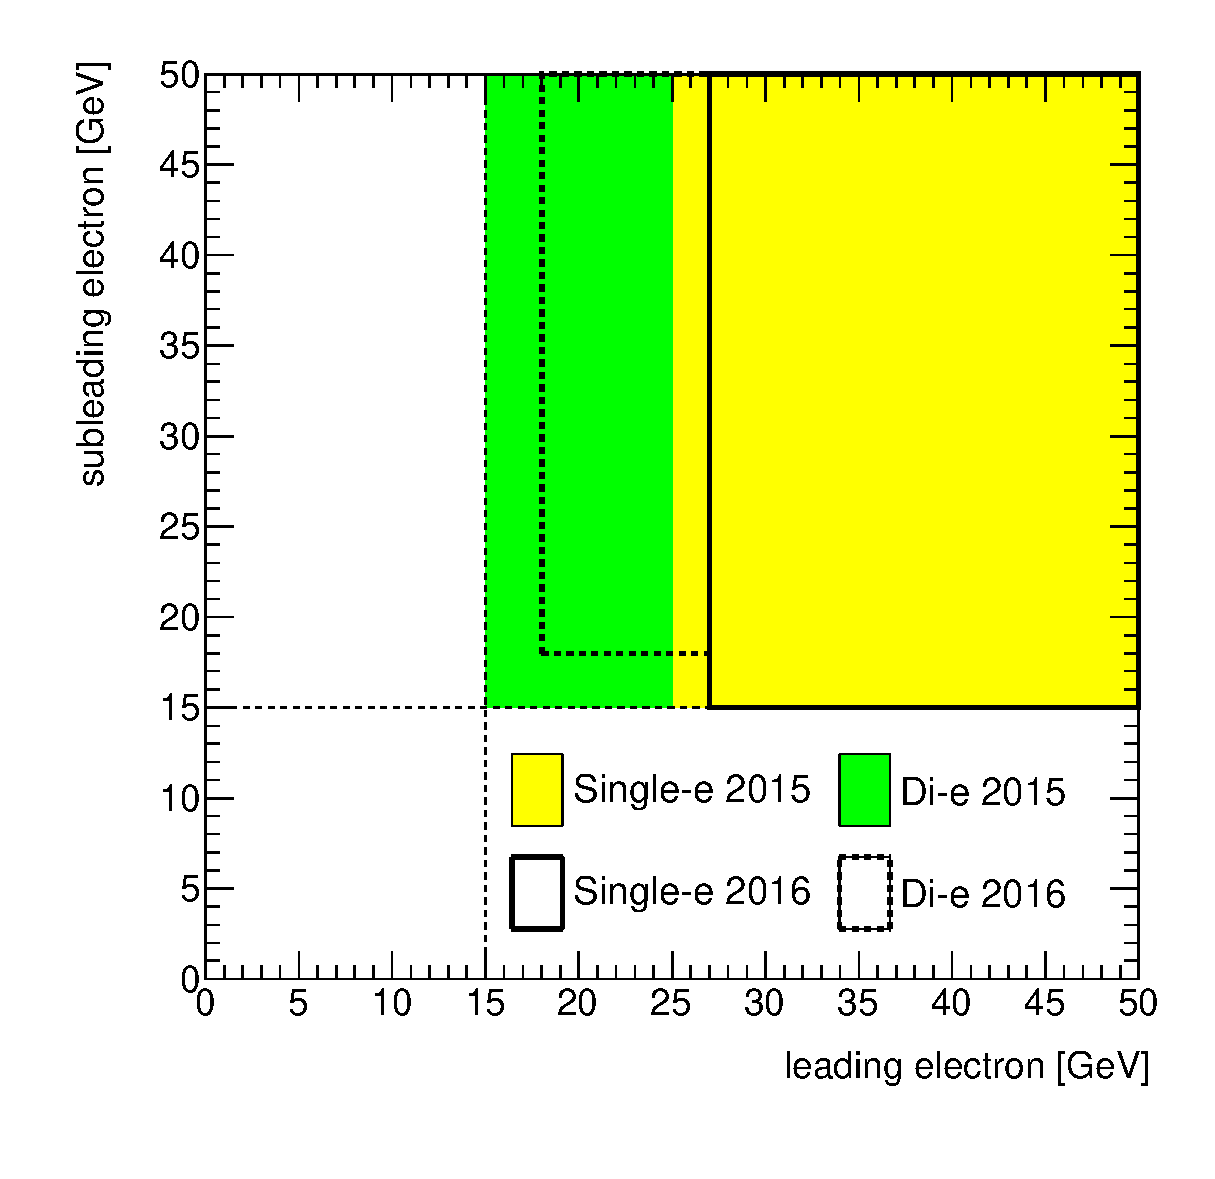
\includegraphics[width=0.3\textwidth]{./figures/event_selection/triggers_ee.eps}
        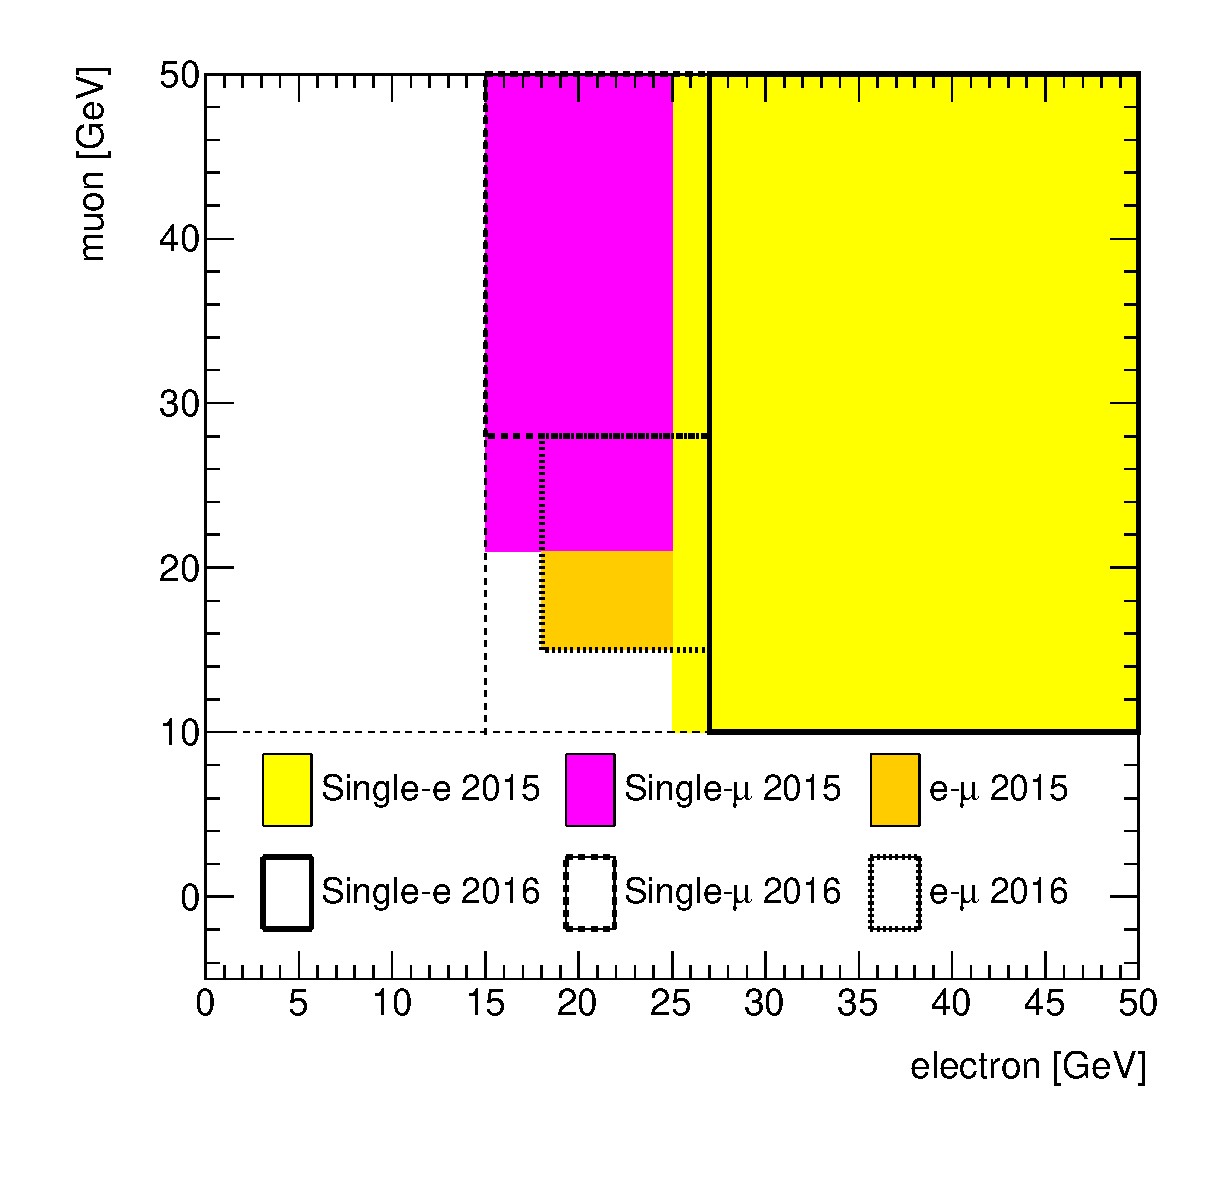
\includegraphics[width=0.3\textwidth]{./figures/event_selection/triggers_emu.eps}
        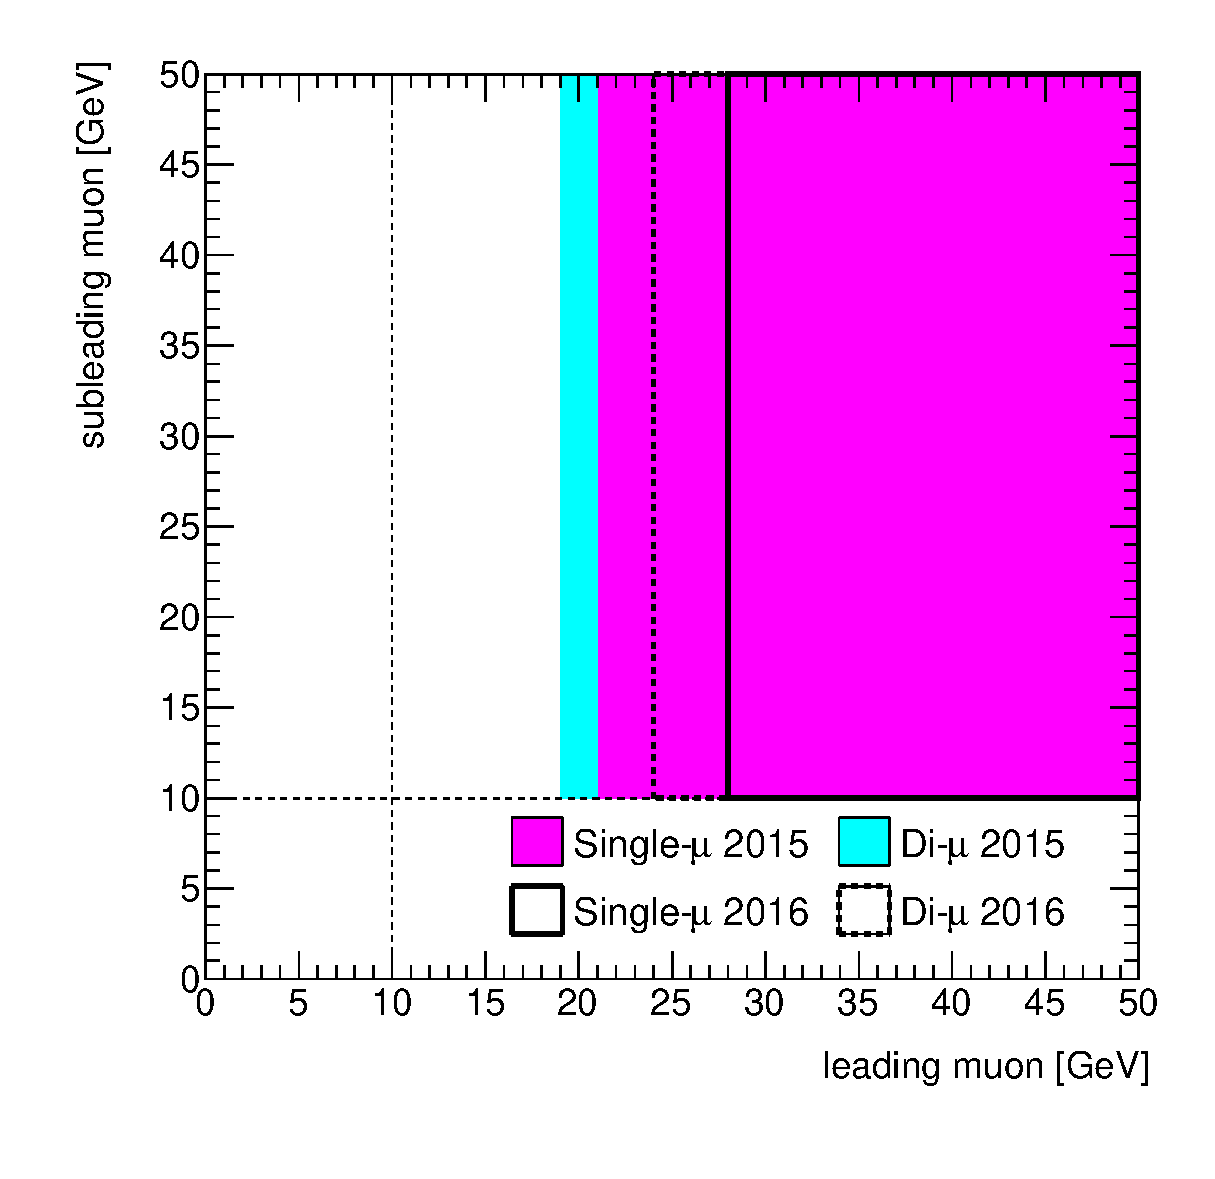
\includegraphics[width=0.3\textwidth]{./figures/event_selection/triggers_mumu.eps}
        \caption{Transverse momentum criteria to select either single-lepton or dilepton triggers in order to avoid overlap.
        The plots correspond to $ee$ (left), $e\mu$ (middle), and $\mu\mu$ (right) final states~\cite{TauConfNote}.}\label{fig:event_selection:triggers}
\end{figure}

Trigger names are composed of a series of acronyms and abbreviations chained together, directly or with underscores,
which define the trigger type and the imposed requirements on the objects to trigger.
For this analysis all trigger names start with \texttt{HLT}, indicating that the software-based High Level Trigger
is used.
Electrons and muons are denoted  as \texttt{e} and \texttt{mu}, respectively, followed by a number defining the transverse
momentum threshold in GeV, which the object has to fulfill.
A preceding number corresponds to multiple objects with the same requirements.
Identification and isolation criteria as introduced in \cref{sec:object_selection:electrons,sec:object_selection:muons}
can be imposed on the triggered objects, which is decoded as \texttt{lhID}
and \texttt{iISO}, where \texttt{ID} and \texttt{ISO} specify the corresponding working points.
If there is no requirement on the distance of the observed tracks to the primary vertex the term \texttt{nod0}
is included.

HLTs can be seeded by L1 triggers, which is indicated by appending the L1 trigger name to to the HLT name.
All L1 trigger names start with \texttt{L1}.
The next part indicates which subdetector fired the L1 trigger.
The electromagnetic calorimeter is referred to as \texttt{EM} and the muon spectrometer as \texttt{MU}.
Next, the transverse energy or transverse momentum threshold in units of GeV is denoted, depending on the subdetector.
The \et{} thresholds can vary slightly as a function of $\eta$, which is denoted with \texttt{V}.
An additional veto on energy depositions in the hadronic calorimeter can be applied, which is indicated by \texttt{H}.

To account for differences in the trigger efficiencies, correction factors are calculated by comparing
the efficiencies between data and simulation~\cite{Trigger2015,Trigger2016}.
An additional offline $\pt$ requirement is introduced to ensure that the trigger efficiencies are in the plateau region.
The thresholds are \SIrange{1}{3}{\GeV} higher than the trigger $\pt$ thresholds.
They can be found in \cref{tab:event_selection:trigger:single,tab:event_selection:trigger:di}.

\section{Preselection}\label{sec:event_selection:preselection}

First, all events are selected which pass the triggers as described in the section above.
Before applying kinematic cuts to suppress background contributions a series of requirements to
ensure data quality are applied.

Data events are discarded if they are not included in the good run list,
which contains the runs where all subdetector systems have been in full operational mode.
The total integrated luminosity of all the good runs in 2015 and 2016 is $\lumiint = \SI{36.1}{\invfb}$.
Additionally, at least one reconstructed vertex consistent with the IP is required.
This rejects events from cosmic rays and beam-halo effects.
Furthermore, badly reconstructed events are removed.

Now basic preselection requirements (\emph{cuts}) are applied to select the decay topology of the \Httll{} decay.
The cuts are enumerated for future references.
In \cref{fig:event_selection:cutflow:1,fig:event_selection:cutflow:2}
distributions of the signal and different backgrounds is shown for a observable before the cut on this observable is performed.
Normalization factors as defined in \cref{sec:background_estimation:normalization} are applied.
Their values are 1,06 for single and pair production of top quarks, and 1.19 and 1.07 for $\Zll$ and $\Ztautau$ production, respectively.
The signal is scaled by factor $50$.
Underflow and overflow bins are included in the first and last bin, respectively.
Only statistical uncertainties are contained in the error band.
\begin{description}[style=nextline,leftmargin=1cm]
    \item[\ \,(1) Number of leptons]
        Exactly two leptons, either two electrons, one electron and on muon, or two muons, with the reconstruction
        and identification criteria defined in \cref{sec:object_selection:electrons,sec:object_selection:muons} are required.
    \item[\ \,(2) Lepton identification and isolation criteria]
        The electrons and muons need to pass the \emph{medium} identification and \emph{gradient} isolation criteria.
    \item[\ \,(3) Hadronic tau veto]
        To ensure orthogonality to the \Httlh{} and \Htthh{} channels all events with one or more hadronic $\tau$-leptons
        obeying the \emph{medium} criterion are vetoed.
    \item[\ \,(4) Trigger]
        The event is associated with the trigger which selected it by testing which trigger is passed by the event.
        Since the trigger efficiency is not the same for data and simulated events, correction factors
        are derived by comparing the trigger efficiency in data and simulation.
        Those correction factors need to be applied to the simulated events.
        However, different triggers have different efficiencies and correction factors, so it is important that the
        correction factor of the right trigger is applied.
    \item[\ \,(5) Trigger matching]
        The objects which caused the event to pass the trigger have to match with the reconstructed leptons.
    \item[\ \,(6) Opposite sign]
        The electric charge of the two leptons has to be opposite.
    \item[\ \,(7) Dilepton mass]
        The mass of the dilepton system is restricted to $\SI{30}{\GeV} < \mll < \SI{75\,(100)}{\GeV}$ for SF (DF) events.
        For SF events this helps to reduce the Drell-Yan $\Zgammall$ background, since the signal distribution peaks at around \SI{50}{\GeV}
        and the $\Zll$ background has its maximum at the mass of the $Z$ boson, $m_Z = \SI{91}{\GeV}$, as shown in \cref{fig:event_selection:cutflow:mllsf}.
        The $\gamma^* \to \ell\ell$ background is reduced by the lower cut, because it rises for low values of $\mll$.
        The main discrimination for DF events is against the top background, which is the dominating background outside of the range spanned by the cut.
        The distribution of $\mll$ for DF events is displayed in \cref{fig:event_selection:cutflow:mlldf}.
    \item[\ \,(8) Jet momentum]
        At least one jet with $\pt > \SI{40}{\GeV}$ is
        required.
        This helps to select both the VBF and boosted category (\cref{sec:event_selection:categorization}).
        The transverse momentum distribution of the leading jet, $\pt^{\text{jet}_1}$, before Cut~8 is shown in \cref{fig:event_selection:cutflow:jetlead}.
        Mainly $\Zll$ and $\Ztautau$ events are rejected by this cut.
    \item[\ \,(9) Missing transverse energy]
        Since the final state includes four neutrinos, a cut on $\etmiss > \SI{20}{\GeV}$ is applied for DF events.
        The $\Zgammall$ background can be suppressed for SF by increasing this cut to $\etmiss > \SI{55}{\GeV}$.
        The distributions for $\etmiss$ before this cut are shwon in \cref{fig:event_selection:cutflow:metsf,fig:event_selection:cutflow:metdf}
        for SF and DF events, respectively.
    \item[(10) Object based missing transverse energy (HPTO)]
        The missing transverse energy is calculated from only high-$\pt$ objects (HPTO). Only the two decay leptons and
        all jets with a transverse momentum of $\pt > \SI{30}{\GeV}$ are used.
        \begin{equation}
            \label{eq:met:hpto}
            \etmissvecobj{\text{HPTO}} = - \ptvec^{\ell_0} - \ptvec^{\ell_1} - \sum_{\mathclap{\substack{\text{jets} \\ \pt > \SI{30}{\GeV}}}} \ptvec^\text{jet}
        \end{equation}
        A HPTO missing transverse energy of $\etmisshpto > \SI{55}{\GeV}$ for SF events is required to further reject
        $\Zgammall$ background, which can be seen in \cref{fig:event_selection:cutflow:hpto}.
    \item[(11) Momentum fraction]
        The momentum fractions carried by the visible decay products of the $\tau$-lepton decay are restricted to $0.1 < x_{1,2} < 1.0$.
        They are calculated in the collinear mass approximation (\cref{sub:event_selection:mcoll}).
        This rejects background events where the assumption of collinearity of the $\tau$-lepton is not met, which leads to
        unphysical solutions.
        \cref{fig:event_selection:cutflow:x1,fig:event_selection:cutflow:x2} show the distributions of $x_1$ and $x_2$ before Cut~11.
    \item[(12) Angular difference in $\bm{\eta}$]
        This cut limits the $\eta$ difference between the two leptons to $\absdetall < 1.5$ to suppress background from single top and top-pair production.
        The $\absdetall$ distribution before Cut~12 is shown in \cref{fig:event_selection:cutflow:detall}.
    \item[(13) Angular difference in $\bm{\dr}$]
        In order to suppress the $\Zll$ and top background, the $\dr$ separation between the two leptons is required to be $\drll < 2$.
        \cref{fig:event_selection:cutflow:drll} shows the $\drll$ distribution before Cut~16.
    \item[(14) Collinear mass]
        To ensure orthogonality with the $H \to WW$ analysis, the collinear mass (\cref{sub:event_selection:mcoll}) is limited to $\mcoll > m_\Z - \SI{25}{\GeV}$.
        Here, a value of $m_\Z = \SI{91.1876}{\GeV}$ is used for the mass of the $Z$ boson.
        The $\mcoll$ distribution before Cut~13 is shown in \cref{fig:event_selection:cutflow:mcoll}.
    \item[(15) MMC mass]
        Events where the MMC mass reconstruction algorithm (\cref{sub:event_selection:mmc}) did not converge are discarded.
    \item[(16) b-jet veto]
        Events which contain $b$-jets (\cref{sec:object_selection:jets}) with $\pt > \SI{25}{\GeV}$ are vetoed.
        This helps to reduce the single-top and $\ttbar$ background.
\end{description}

\begin{figure}[htb]
    \centering
    \begin{subfigure}[t]{0.45\textwidth}
        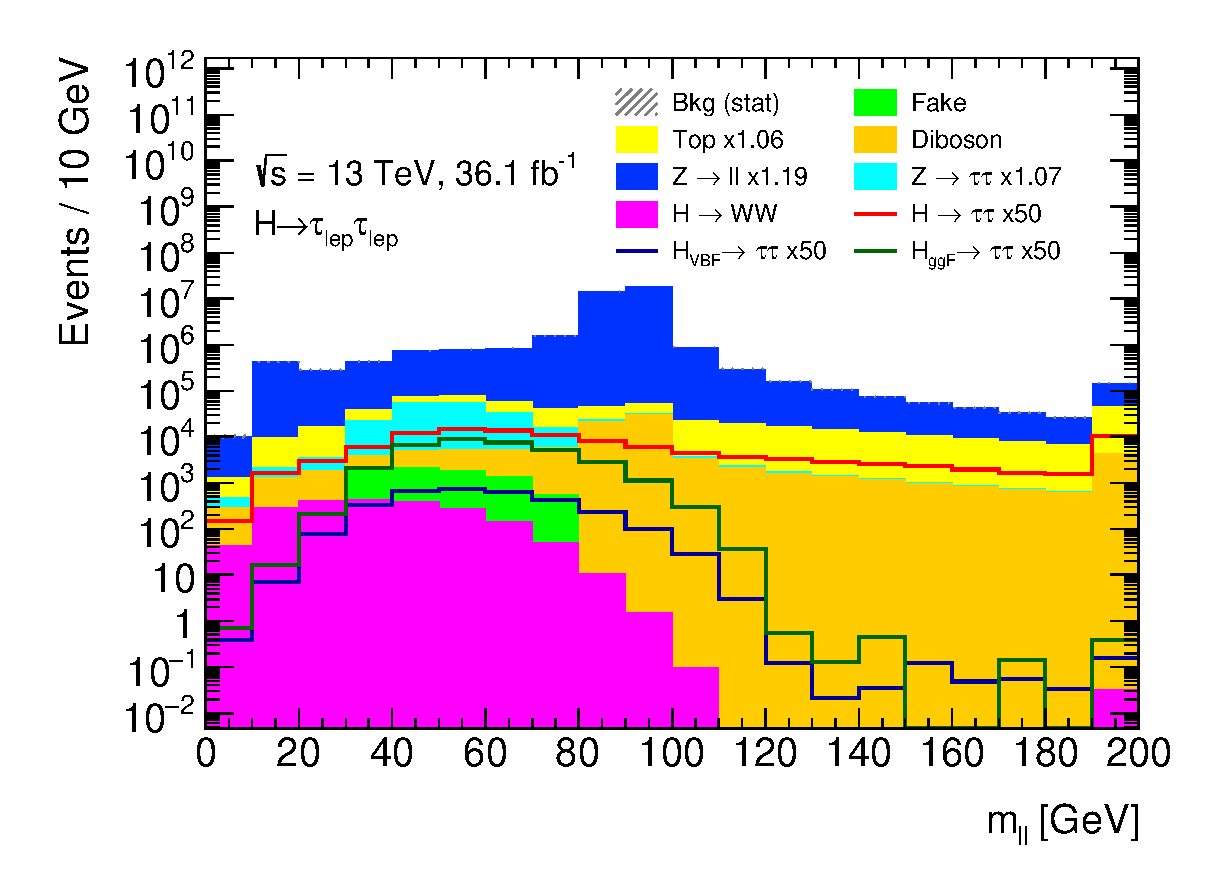
\includegraphics[width=\textwidth]{./plots/event_selection/presel/eemm-CutOS-mvis-log.eps}
        \caption{}\label{fig:event_selection:cutflow:mllsf}
    \end{subfigure}
    \begin{subfigure}[t]{0.45\textwidth}
        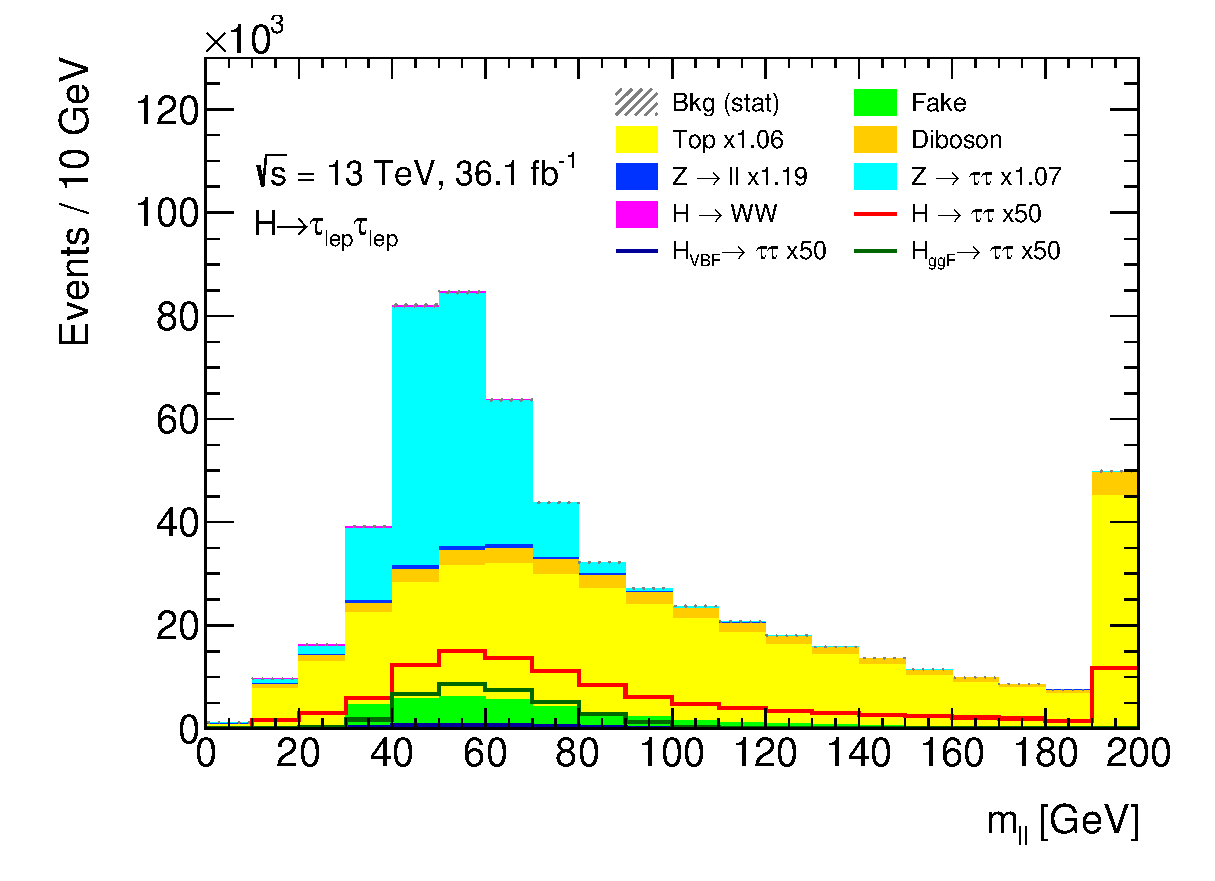
\includegraphics[width=\textwidth]{./plots/event_selection/presel/emme-CutOS-mvis-lin.eps}
        \caption{}\label{fig:event_selection:cutflow:mlldf}
    \end{subfigure}
    \begin{subfigure}[t]{0.45\textwidth}
        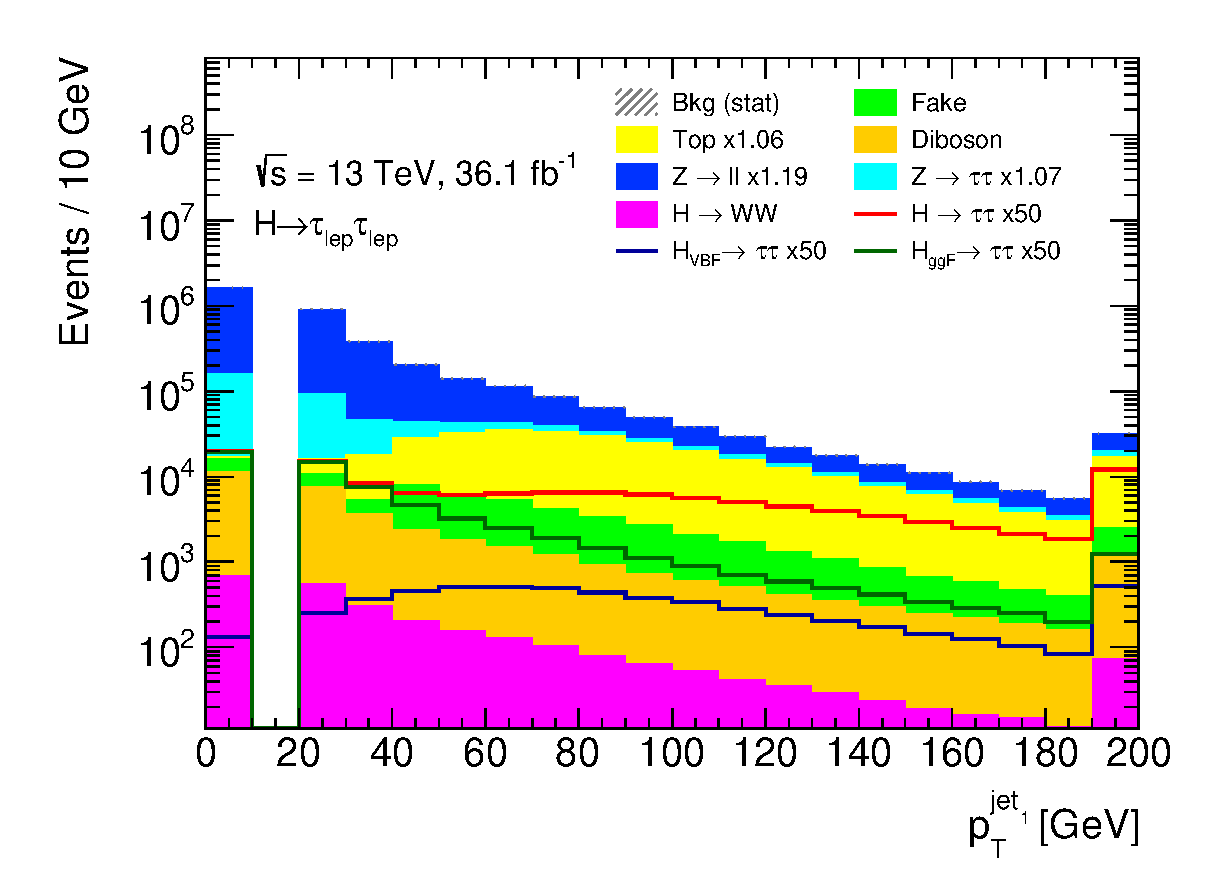
\includegraphics[width=\textwidth]{./plots/event_selection/presel/ll-CutMVis-JetPt0-log.eps}
        \caption{}\label{fig:event_selection:cutflow:jetlead}
    \end{subfigure}
    \begin{subfigure}[t]{0.45\textwidth}
        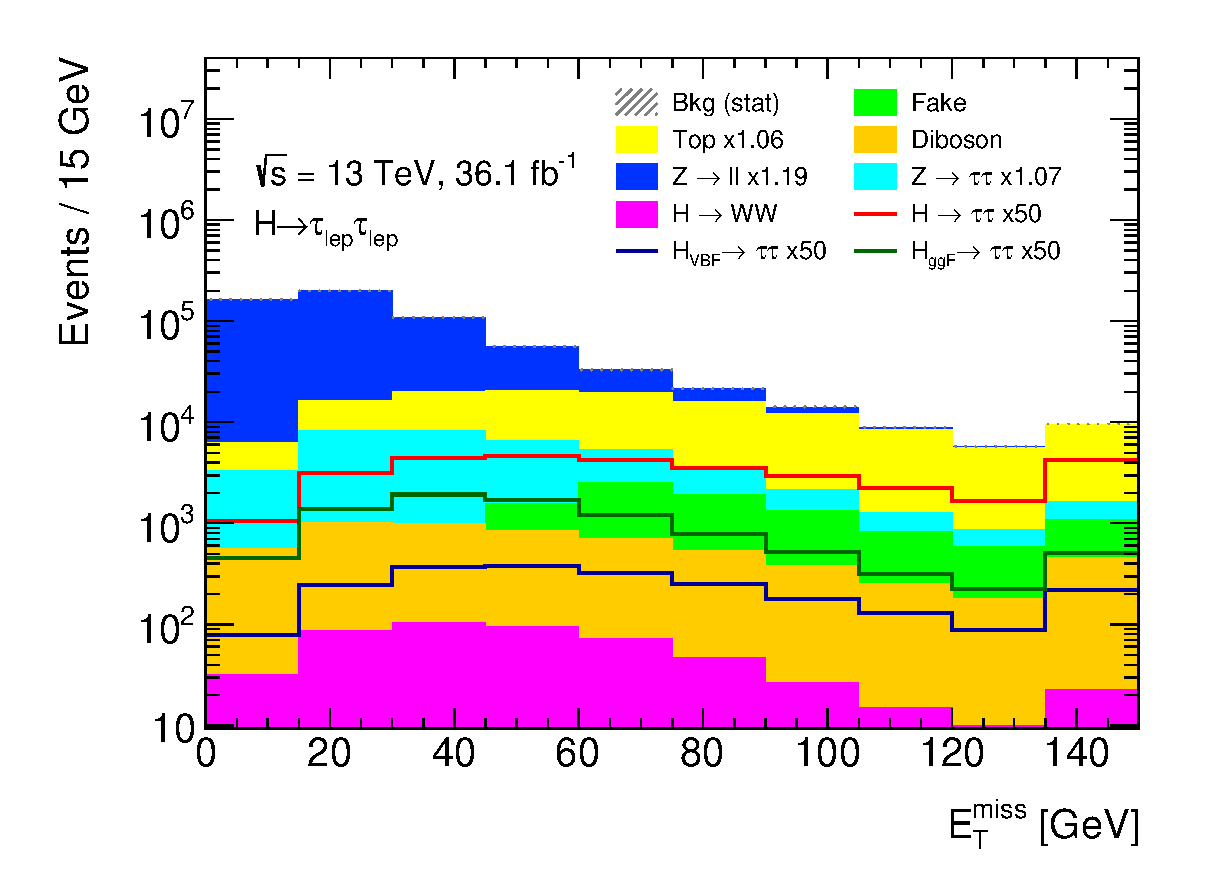
\includegraphics[width=\textwidth]{./plots/event_selection/presel/eemm-CutJet0Pt-MET-log.eps}
        \caption{}\label{fig:event_selection:cutflow:metsf}
    \end{subfigure}
    \begin{subfigure}[t]{0.45\textwidth}
        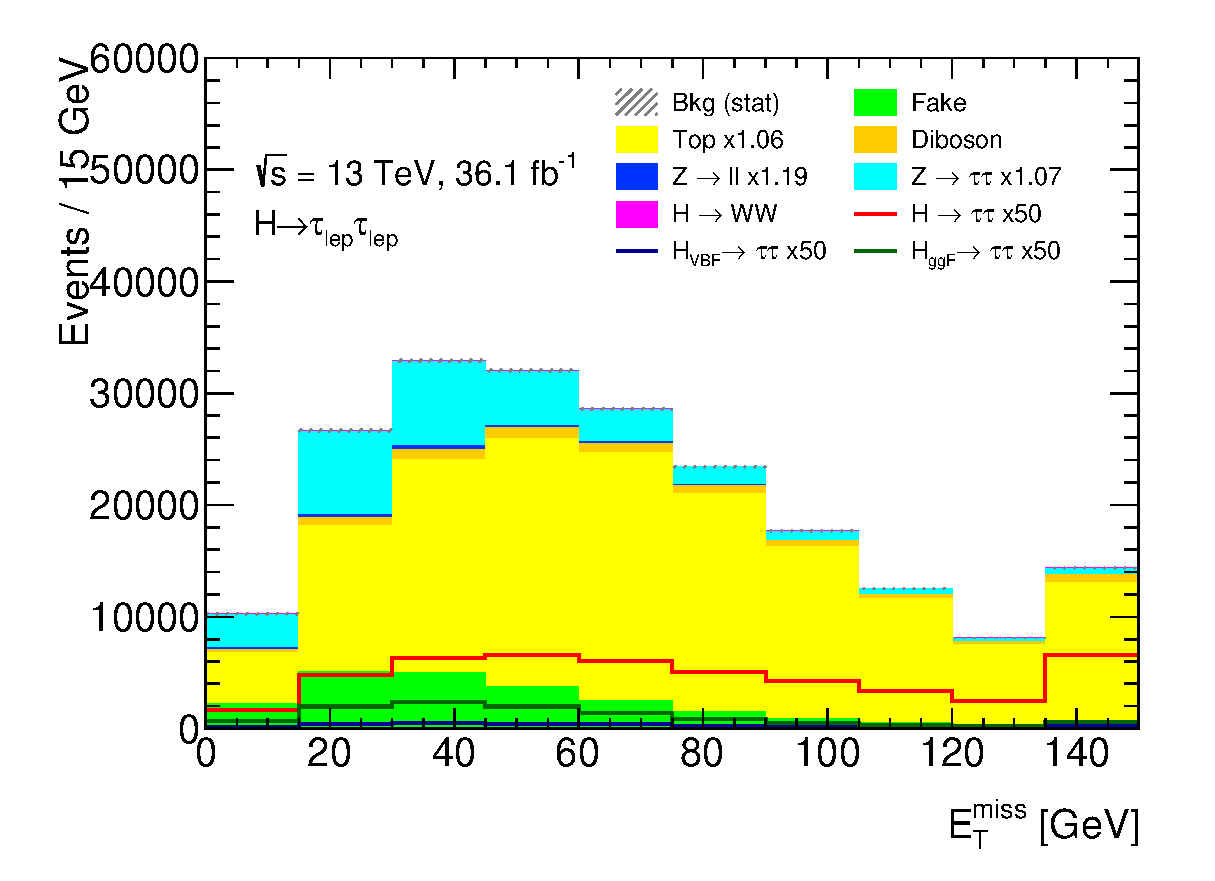
\includegraphics[width=\textwidth]{./plots/event_selection/presel/emme-CutJet0Pt-MET-lin.eps}
        \caption{}\label{fig:event_selection:cutflow:metdf}
    \end{subfigure}
    \begin{subfigure}[t]{0.45\textwidth}
        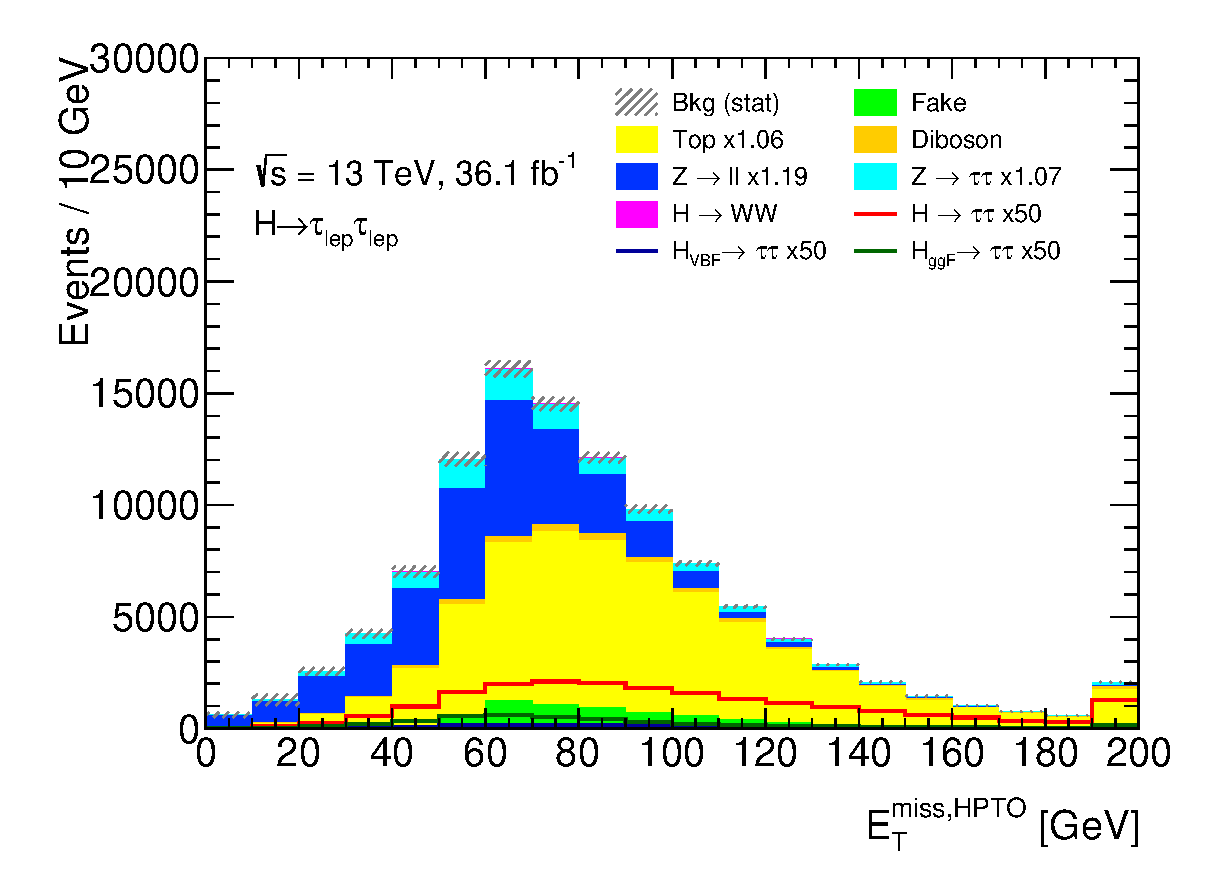
\includegraphics[width=\textwidth]{./plots/event_selection/presel/eemm-CutMET-METhpto-lin.eps}
        \caption{}\label{fig:event_selection:cutflow:hpto}
    \end{subfigure}
    \caption{Distribution of several observables which are used in the preselection before the corresponding cut is applied.
             The following observables are shown: $\mll$ for SF events after Cut~6 (a), $\mll$ for DF events after Cut~6 (b), $\pt^{\text{jet}_1}$ after Cut~7 (c),
             $\etmiss$ for SF events after Cut~8 (d), $\etmiss$ for DF events after Cut~8 (e), and $\etmisshpto$ for SF events after Cut~9 (e).
             The signal and background distributions are normalized to their theory cross-section and luminosity.
             Additional normalization factors are applied on the top-quark, $\Zll$, and $\Ztautau$ background.
             The signal is scaled by a factor of 50.
             Underflow and overflow bins are included in the first and last bin, respectively.
             Only statistical uncertainties are included in the error band.}\label{fig:event_selection:cutflow:1}
\end{figure}

\begin{figure}[htb]
    \centering
    \begin{subfigure}[t]{0.45\textwidth}
        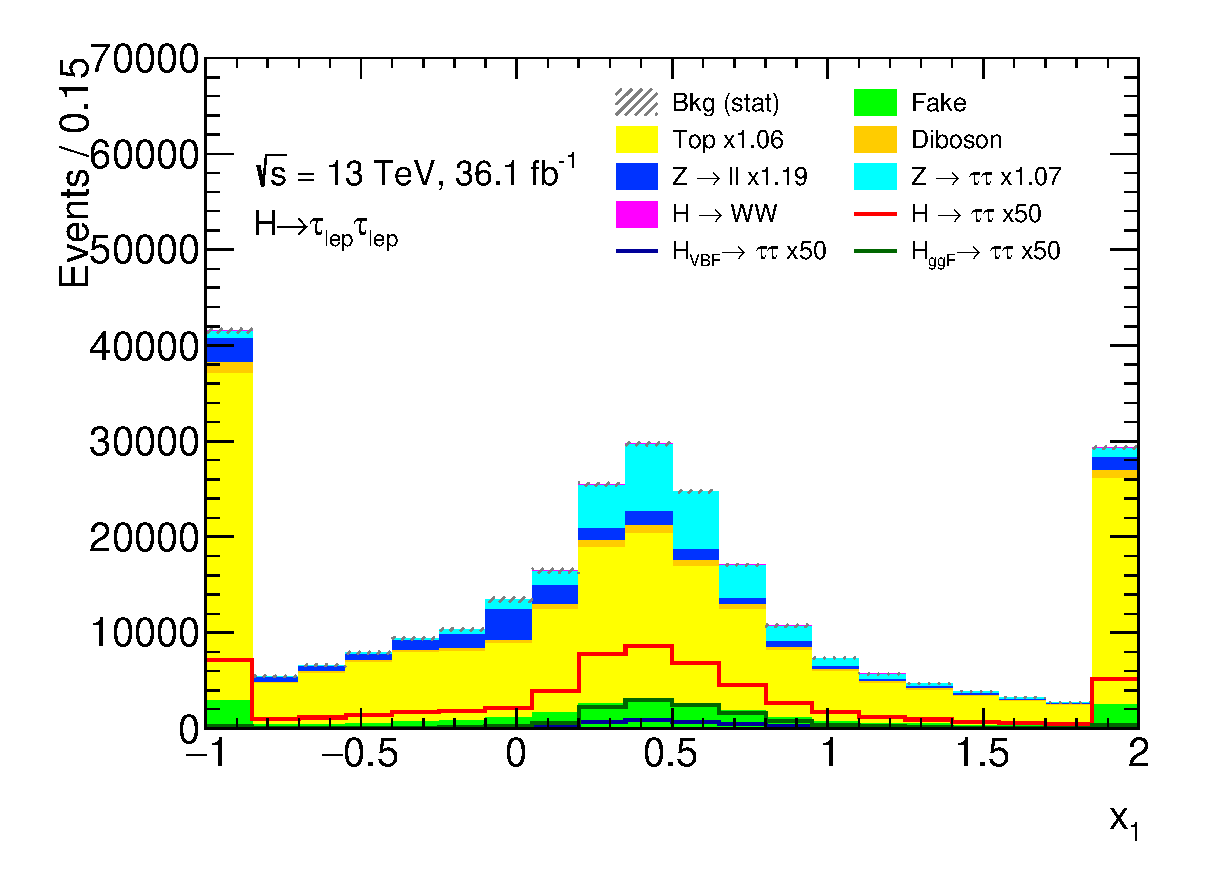
\includegraphics[width=\textwidth]{./plots/event_selection/presel/ll-CutHPTO-x0wide-lin.eps}
        \caption{}\label{fig:event_selection:cutflow:x1}
    \end{subfigure}
    \begin{subfigure}[t]{0.45\textwidth}
        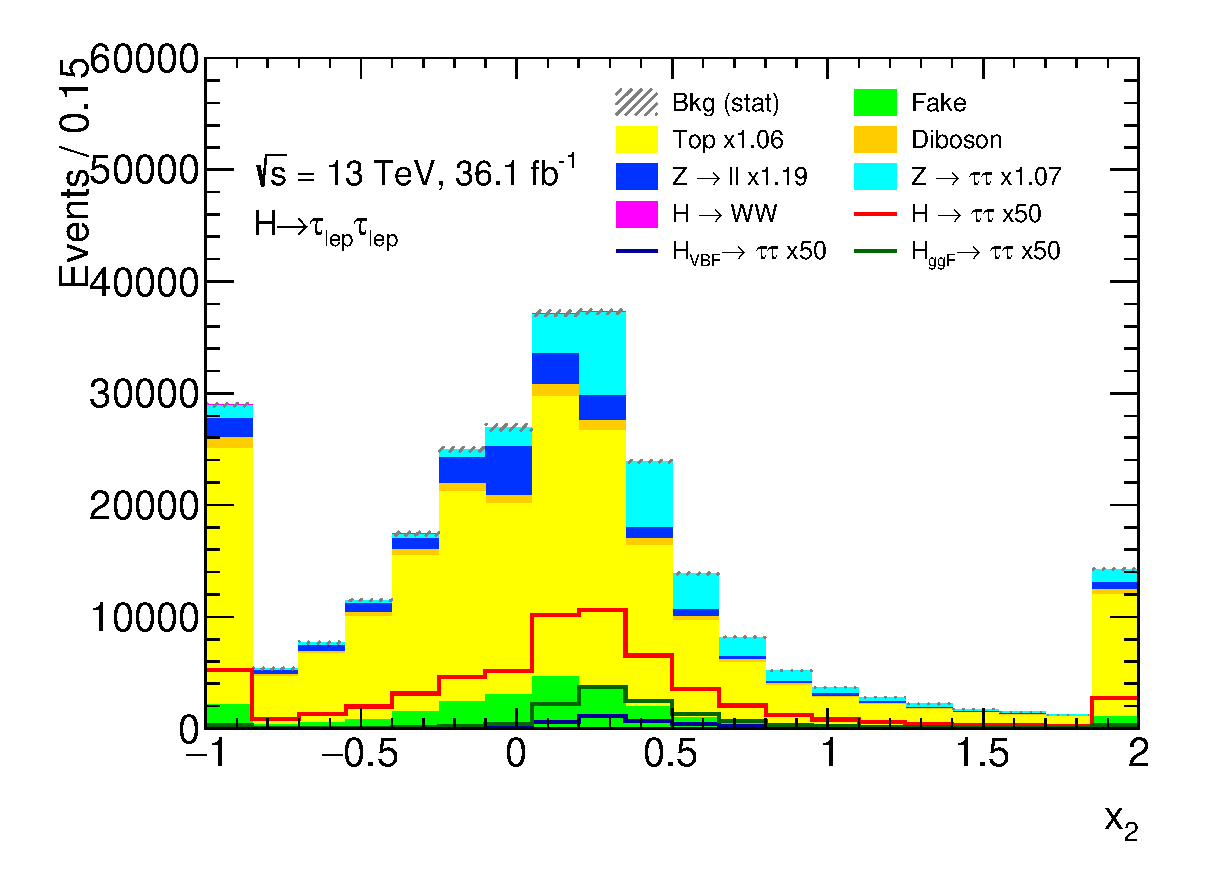
\includegraphics[width=\textwidth]{./plots/event_selection/presel/ll-CutHPTO-x1wide-lin.eps}
        \caption{}\label{fig:event_selection:cutflow:x2}
    \end{subfigure}
    \begin{subfigure}[t]{0.45\textwidth}
        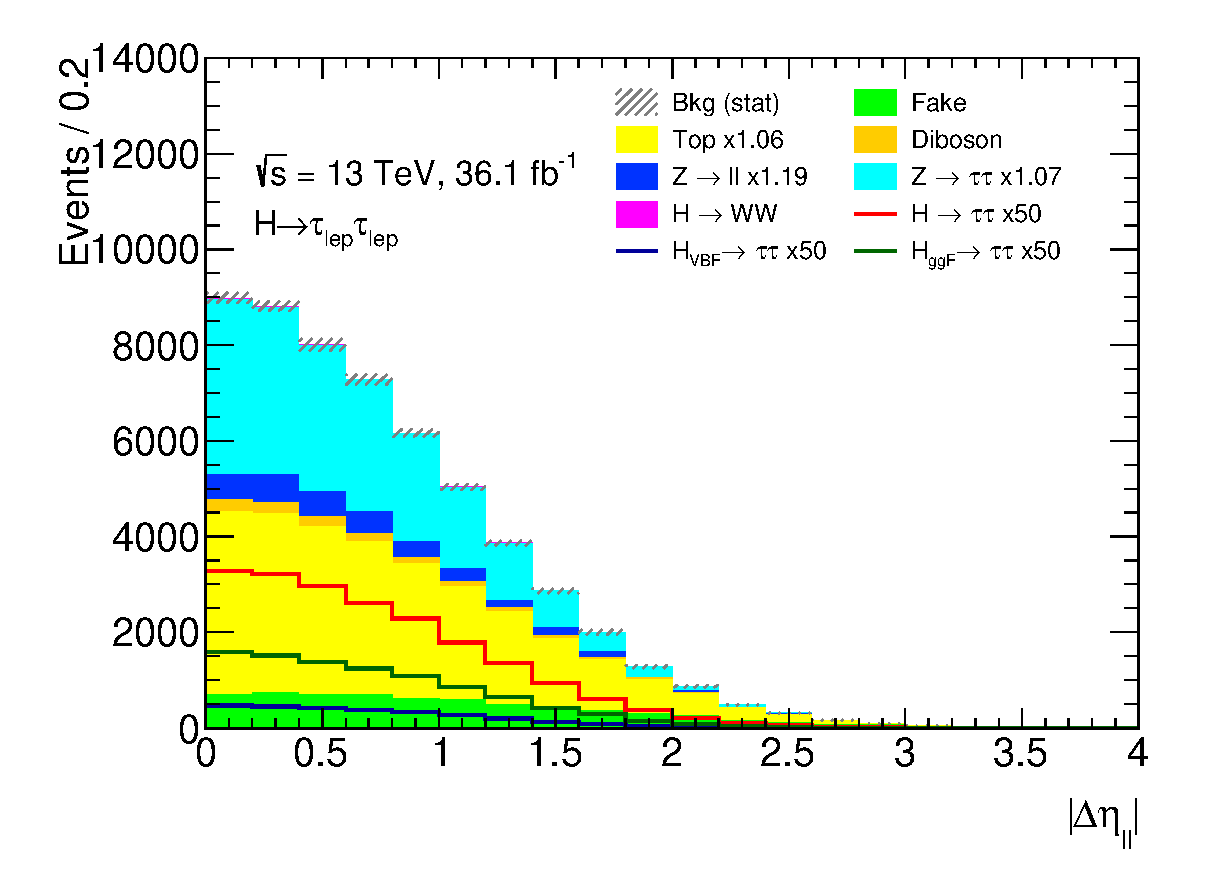
\includegraphics[width=\textwidth]{./plots/event_selection/presel/ll-CutX-DeltaEtaLL-lin.eps}
        \caption{}\label{fig:event_selection:cutflow:detall}
    \end{subfigure}
    \begin{subfigure}[t]{0.45\textwidth}
        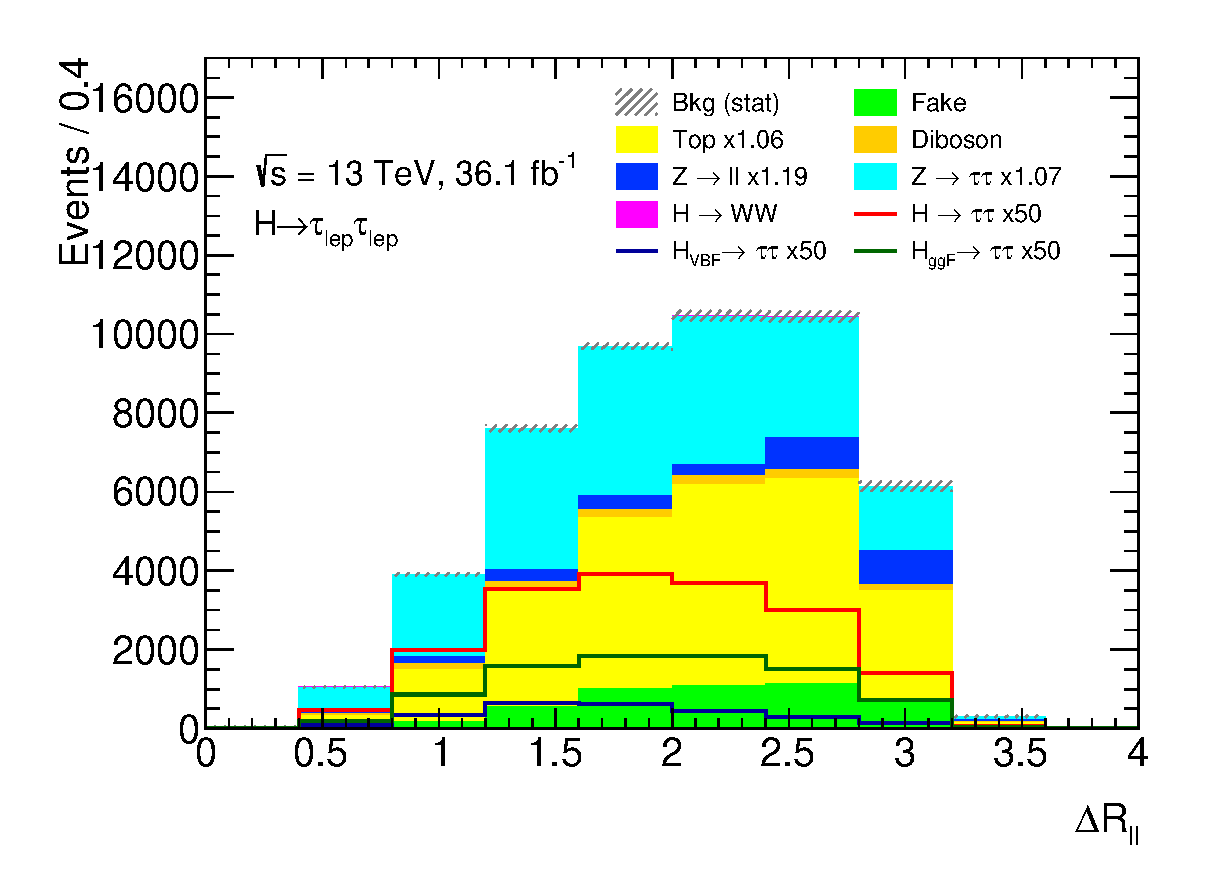
\includegraphics[width=\textwidth]{./plots/event_selection/presel/ll-CutDEtaLL-DeltaRLL-lin.eps}
        \caption{}\label{fig:event_selection:cutflow:drll}
    \end{subfigure}
    \begin{subfigure}[t]{0.45\textwidth}
        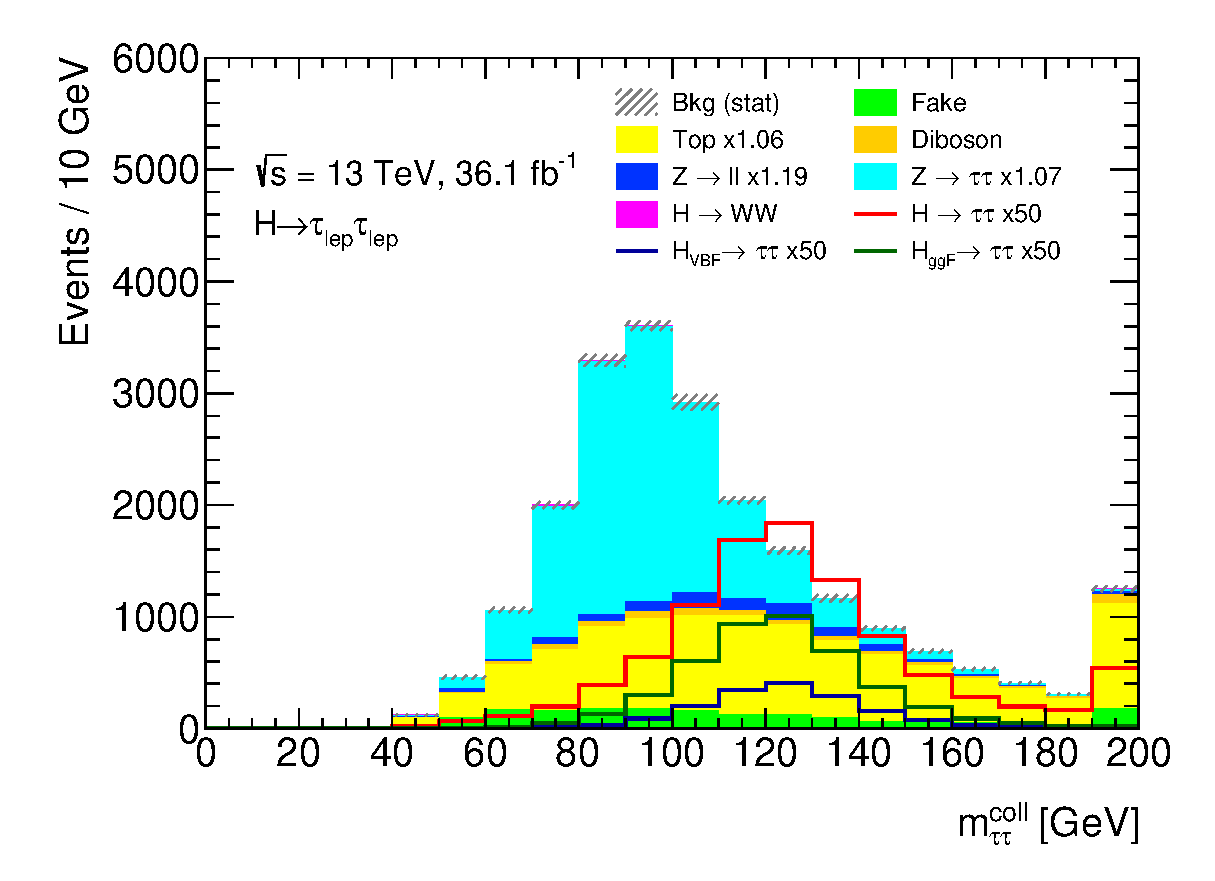
\includegraphics[width=\textwidth]{./plots/event_selection/presel/ll-CutDRLL-mcoll-lin.eps}
        \caption{}\label{fig:event_selection:cutflow:mcoll}
    \end{subfigure}
    \caption{Distribution of several observables which are used in the preselection before the corresponding cut is applied.
             The following observables are shown: $x_1$ after Cut~10, $x_2$ after Cut~10, $\absdetall$ after Cut~11, $\drll$ after Cut~12, and $\mcoll$ after Cut~13.
             The signal and background distributions are normalized to their theory cross-section and luminosity.
             Additional normalization factors are applied on the top-quark, $\Zll$, and $\Ztautau$ background.
             The signal is scaled by a factor of 50.
             Underflow and overflow bins are included in the first and last bin, respectively.
             Only statistical uncertainties are included in the error band.}\label{fig:event_selection:cutflow:2}
\end{figure}


\section{Categorization}\label{sec:event_selection:categorization}

Since the goal of this analysis is to measure the coupling strength of the Higgs boson
in different production modes, dedicated categories for the VBF and gluon--gluon fusion production mode
are defined by exploiting production-mode specific event topologies.
They are referred to as the \emph{VBF} and \emph{boosted category}, respectively.
The signal-to-background ratio and background composition is different in those categories.
Due to the splitting the overall sensitivity of the measurement is enhanced.
Further subcategories formed in both cases to improve the sensitivity even more.

\subsection{VBF category}\label{sub:event_selection:vbf}

In the VBF production mode two vector bosons are used to produce the Higgs boson.
The vector bosons originate from two partons, which produce two jets with high transverse momentum
in the forward and backward region of the detector.
Small jet activity is expected between the two VBF jets, because there is no color flow between the initial partons.
The following cuts are applied to select this topology:

\begin{itemize}
    \item Subleading jet momentum (Cut 1V) \\
        A second jet is required with at least $\pt > \SI{30}{\GeV}$, because the VBF topology has two jets.
        \cref{fig:event_selection:cutflow:vbf:jet2} shows the distribution of the transverse momentum of the second
        jet before this cut.
    \item Opposite hemispheres (Cut 2V) \\
        The two leading jets most likely occupy different hemispheres of the detector due to the VBF topology.
        This can be achieved by applying the $\eta_{\text{jet}_1} \cdot \eta_{\text{jet}_2} < 0$ requirement.
        The distribution of $\eta_{\text{jet}_1} \cdot \eta_{\text{jet}_2}$ before Cut~2V is shown in \cref{fig:event_selection:cutflow:vbf:hemispheres}.
    \item Angular separation of two leading jets (Cut 3V) \\
        The separation in $\eta$ between the two VBF jets is expected to be large, as shown in \cref{fig:event_selection:cutflow:vbf:detajj}.
        Therefore, a cut of $\absdetajj > 3$ is applied.
    \item Lepton candidate centrality (Cut 4V) \\
        The $\eta$ of the selected leptons must lie in between the two jets.
    \item Invariant mass of the dijet system (Cut 5V) \\
        The dijet system is required to have an invariant mass of $\mjj > \SI{400}{\GeV}$.
        The distribution of $\mjj$ before Cut~5V is shown in \cref{fig:event_selection:cutflow:vbf:mjj}.
\end{itemize}

Furthermore, the VBF category is split into a \emph{high} and \emph{low} VBF category,
with requirements on the transverse momentum of the di-$\tau$ system, $\pt^{\tau\tau} > \SI{100}{\GeV}$ and $\pt^{\tau\tau} < \SI{100}{\GeV}$, respectively.
The transverse momentum of the di-$\tau$ system is calculated from the transverse momenta of the visible decay products of the
$\tau$-leptons and the missing transverse energy.
This helps to increase the sensitivity, provided that the statistics in the subcategories are still high enough.

%The distributions of $\mmc$ in the inclusive, high, and low VBF category is shown in \cref{fig:event_selection:vbf:mmc}.

% \begin{figure}[htb]
%     \centering
%     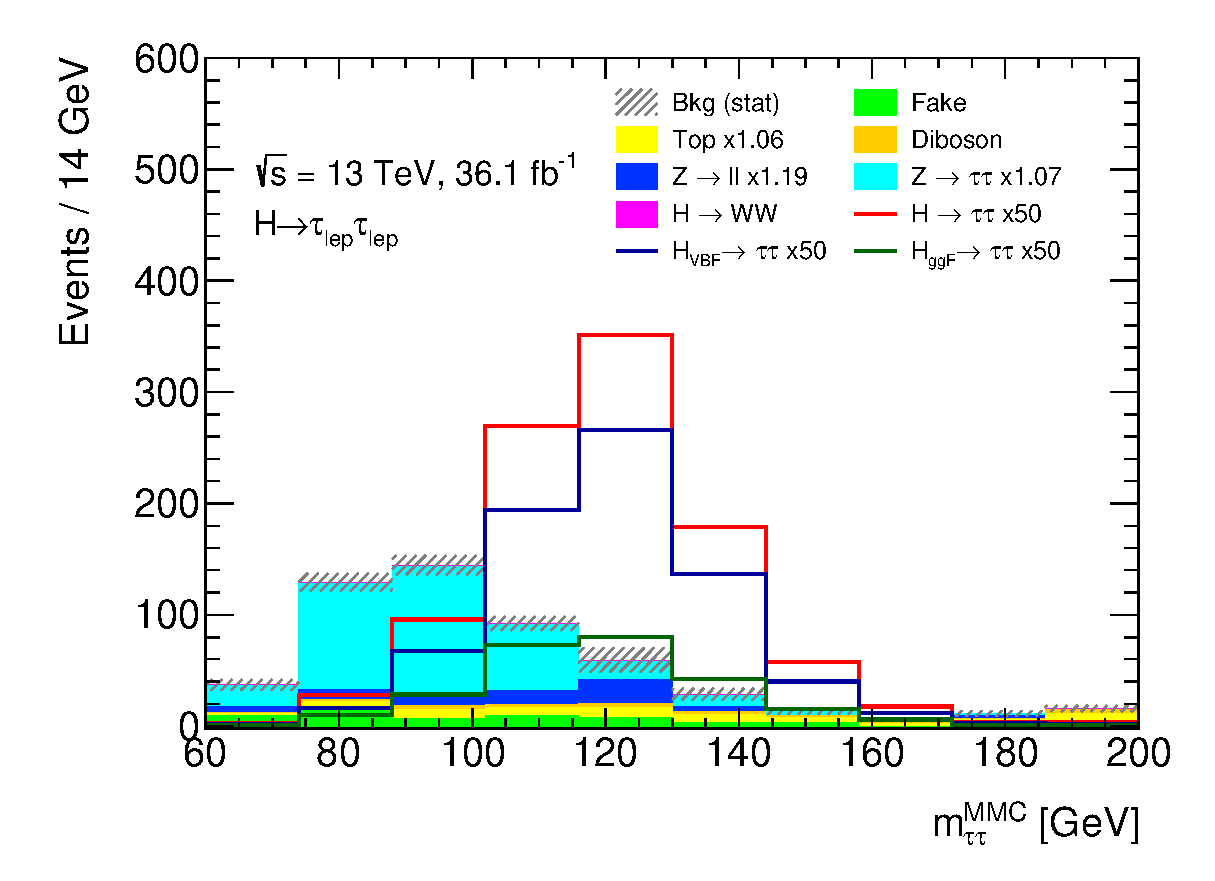
\includegraphics[width=0.3\textwidth]{./plots/event_selection/presel/ll-CutVBFCatMjj-dilep_mmc_mlm_m_vbf-lin.eps}
%     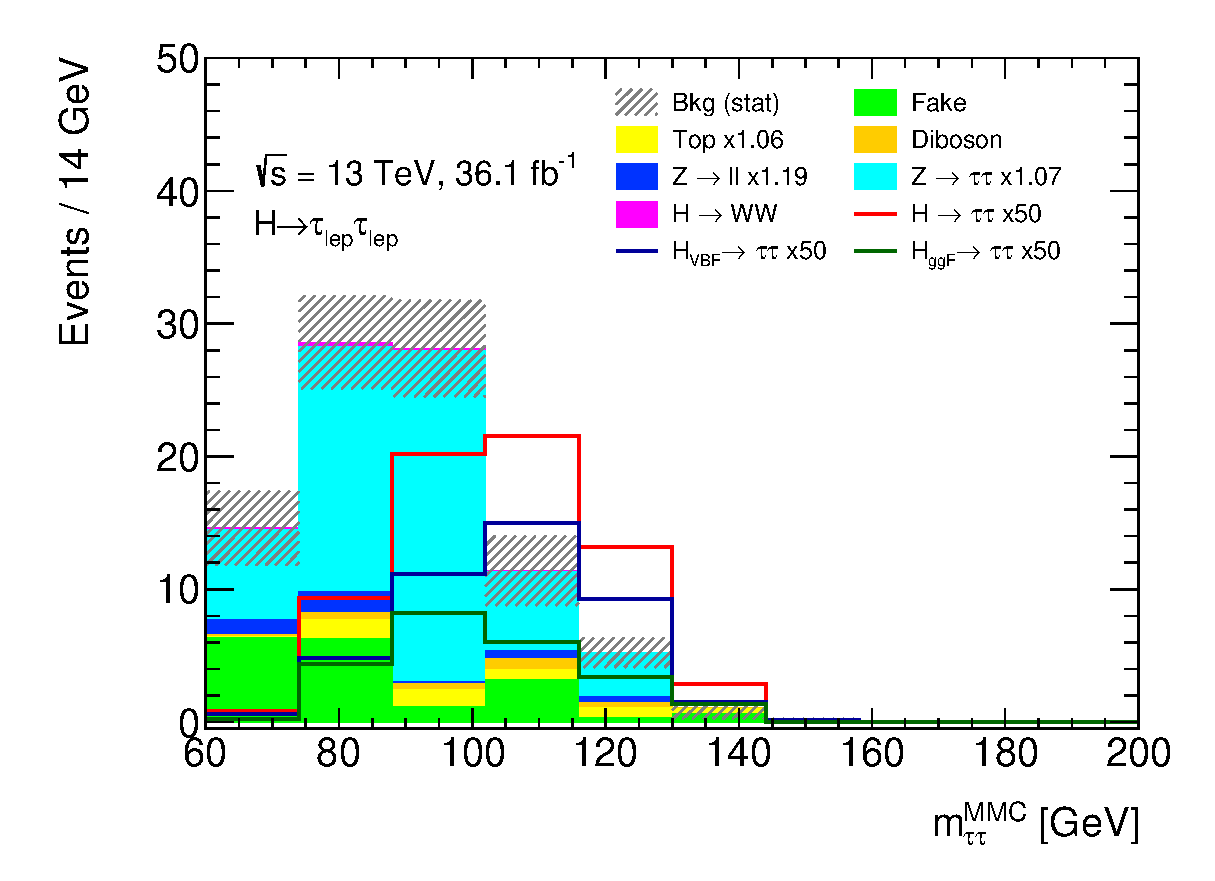
\includegraphics[width=0.3\textwidth]{./plots/event_selection/presel/ll-CutVBFCatA-dilep_mmc_mlm_m_vbf-lin.eps}
%     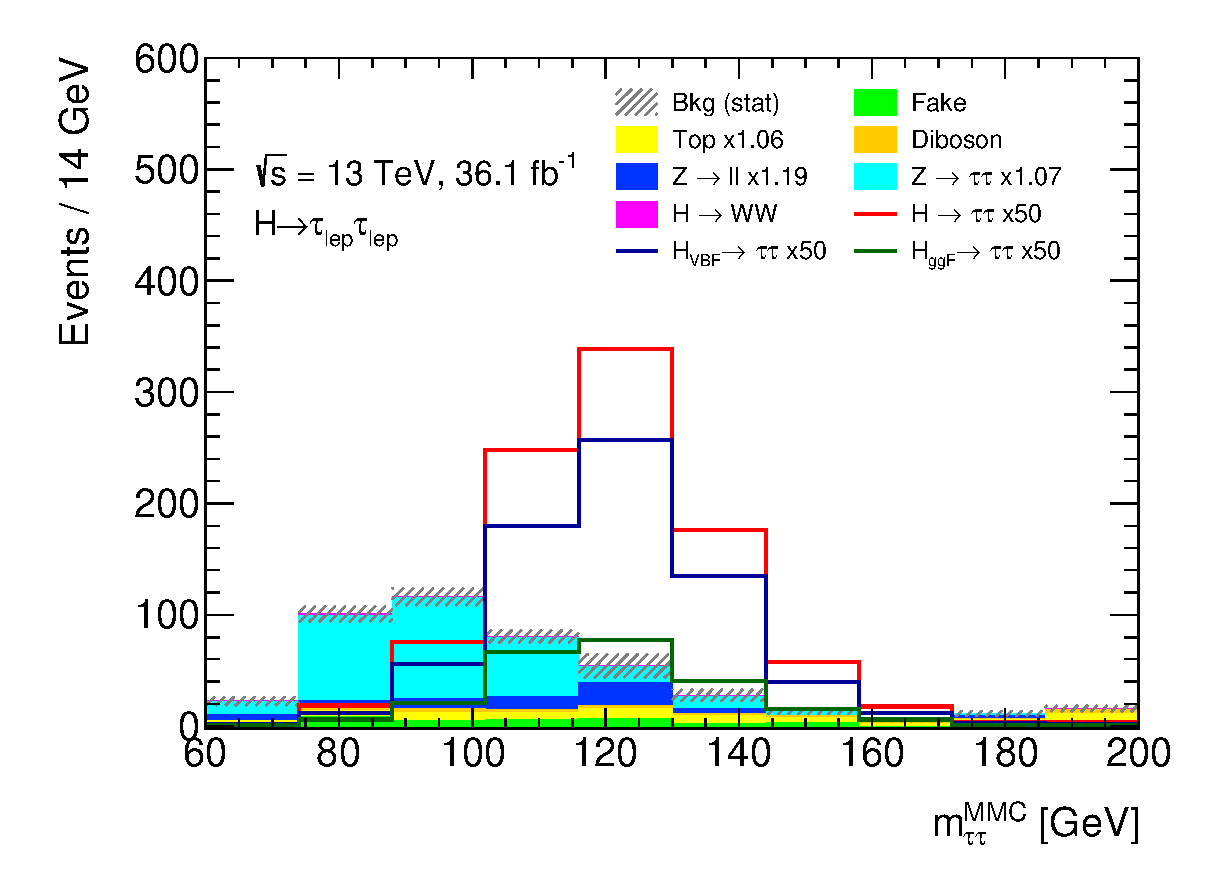
\includegraphics[width=0.3\textwidth]{./plots/event_selection/presel/ll-CutVBFCatB-dilep_mmc_mlm_m_vbf-lin.eps}
%     \caption{Distributions of the output of the missing mass calculator algorithm, $\mmc$, in the inclusive (left),
%              low (middle), and high (right) VBF category.
%              Normalization factors are applied on the top-quark, $\Zll$, and $\Ztautau$ background.
%              The signal is scaled by a factor of 20.
%              The error band includes statistic and systematic uncertainties.}\label{fig:event_selection:vbf:mmc}
% \end{figure}

\subsection{Boosted category}\label{sub:event_selection:boosted}

In contrast to the VBF production mode, the gluon--gluon fusion production mode has no outgoing partons at tree-level.
However, higher order QCD corrections can produce one or more jets, which leads to a high transverse momentum of the Higgs boson.
An example Feynman diagram for such a process is displayed in \cref{fig:event_selection:boostedjet}.

\begin{figure}[htb]
    \centering
    \includegraphics[width=0.5\textwidth]{./feynman/boosted.pdf}
    \caption{Production of a Higgs boson via gluon--gluon fusion with an additional jet.}\label{fig:event_selection:boostedjet}
\end{figure}


The selection criteria for the boosted category are as follows:
\begin{itemize}
    \item Veto on VBF selection (Cut 1B)
        The events have to pass the preselection, but not the VBF selection.
    \item Higgs boson transverse momentum (Cut 2B)
        The transverse momentum of the di-$\tau$ system is required to be $\pt^{\tau\tau} > \SI{100}{\GeV}$, since
        the goal is to select the boosted topology.
        A distribution of $\pt^{\tau\tau}$ before Cut~2B is shown in \cref{fig:event_selection:cutflow:boosted:pttautau}.
\end{itemize}
Similar to the VBF category, also the boosted category is divided into two subcategories.
All events which pass the requirements $\pt^{\tau\tau} > \SI{140}{\GeV}$ and $\drll < 1.5$ are sorted
into the \emph{high-boosted} category. All other events which do not pass these criteria are filled in the
\emph{low-boosted} category.

\begin{figure}[htb]
    \centering
    \begin{subfigure}[t]{0.45\textwidth}
        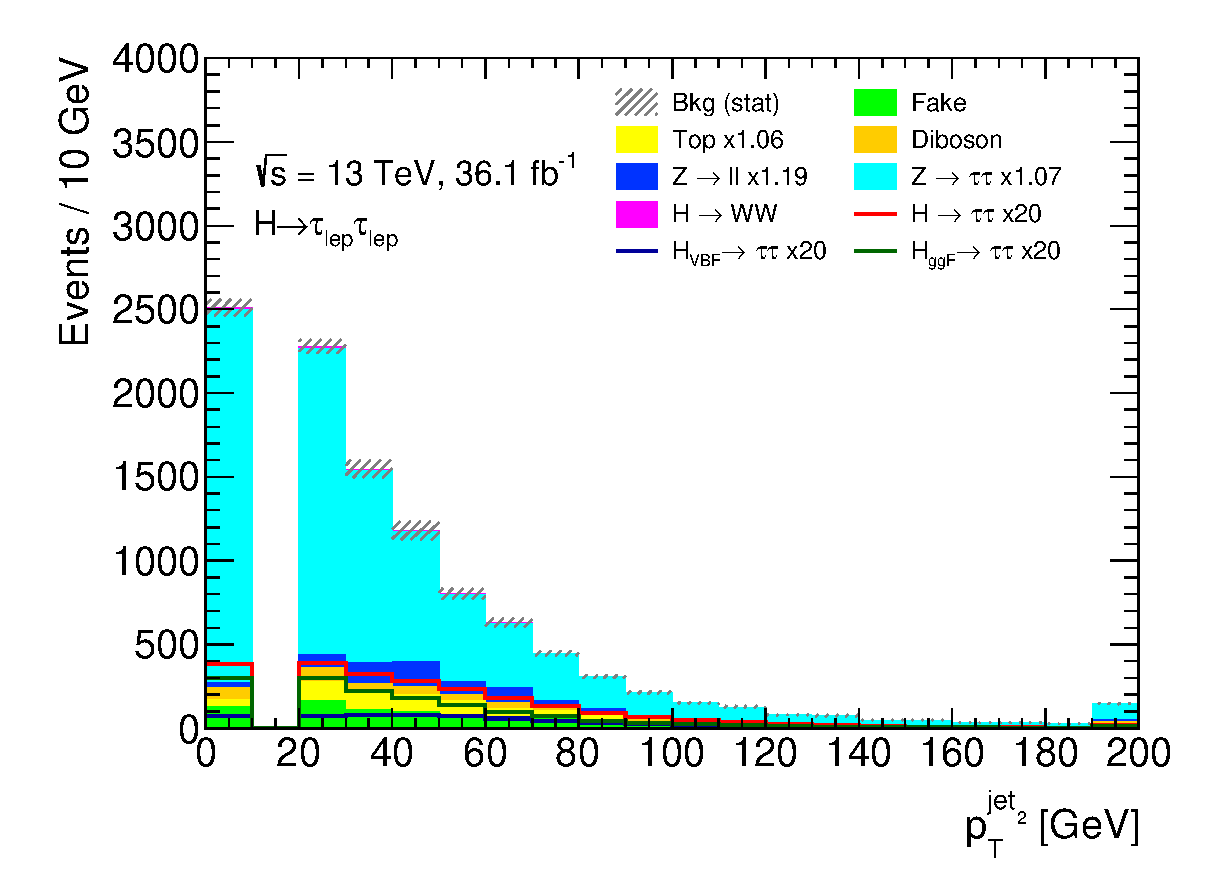
\includegraphics[width=\textwidth]{./plots/event_selection/categories/ll-CutbVeto-JetPt1-lin.eps}
        \caption{}\label{fig:event_selection:cutflow:vbf:jet2}
    \end{subfigure}
    \begin{subfigure}[t]{0.45\textwidth}
        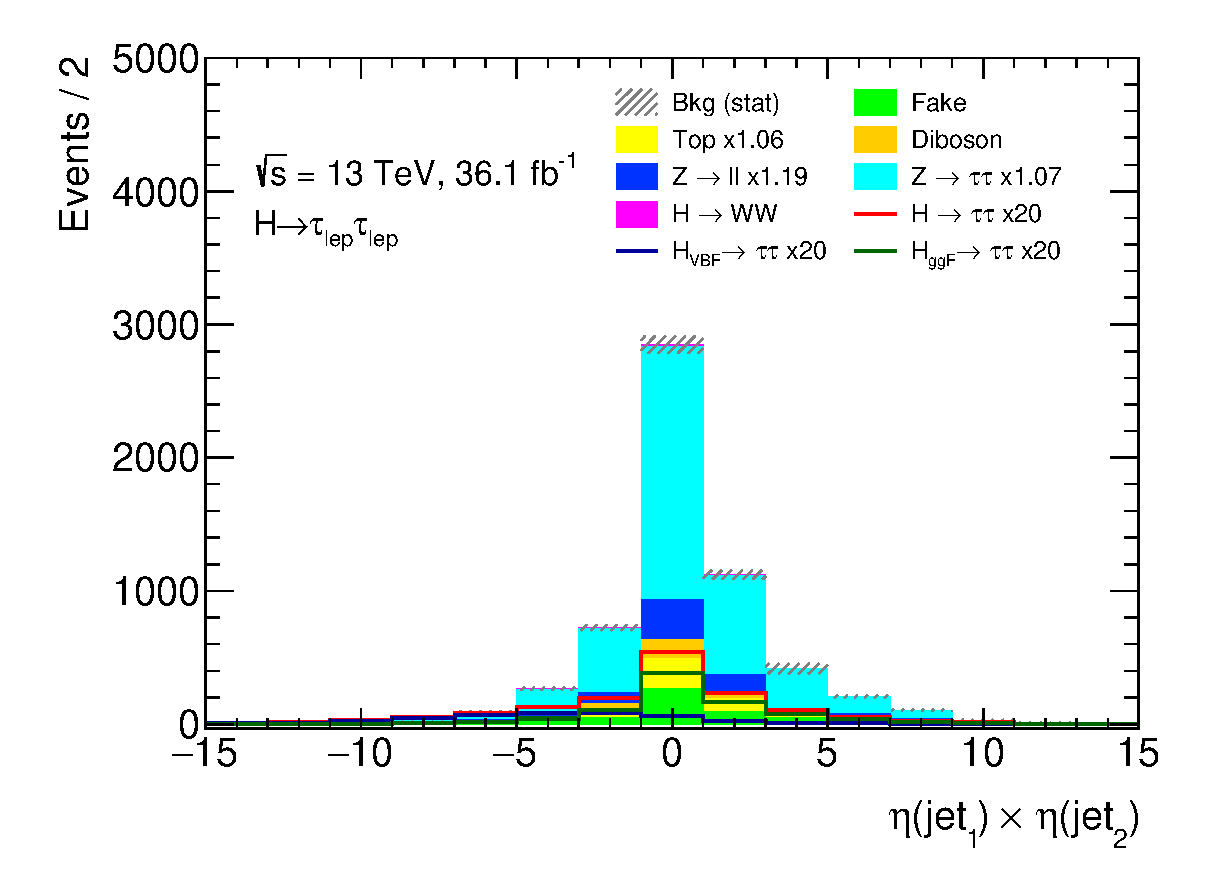
\includegraphics[width=\textwidth]{./plots/event_selection/categories/ll-CutVBFCatJet1Pt-EtaProductJ0J1-lin.eps}
        \caption{}\label{fig:event_selection:cutflow:vbf:hemispheres}
    \end{subfigure}
    \begin{subfigure}[t]{0.45\textwidth}
        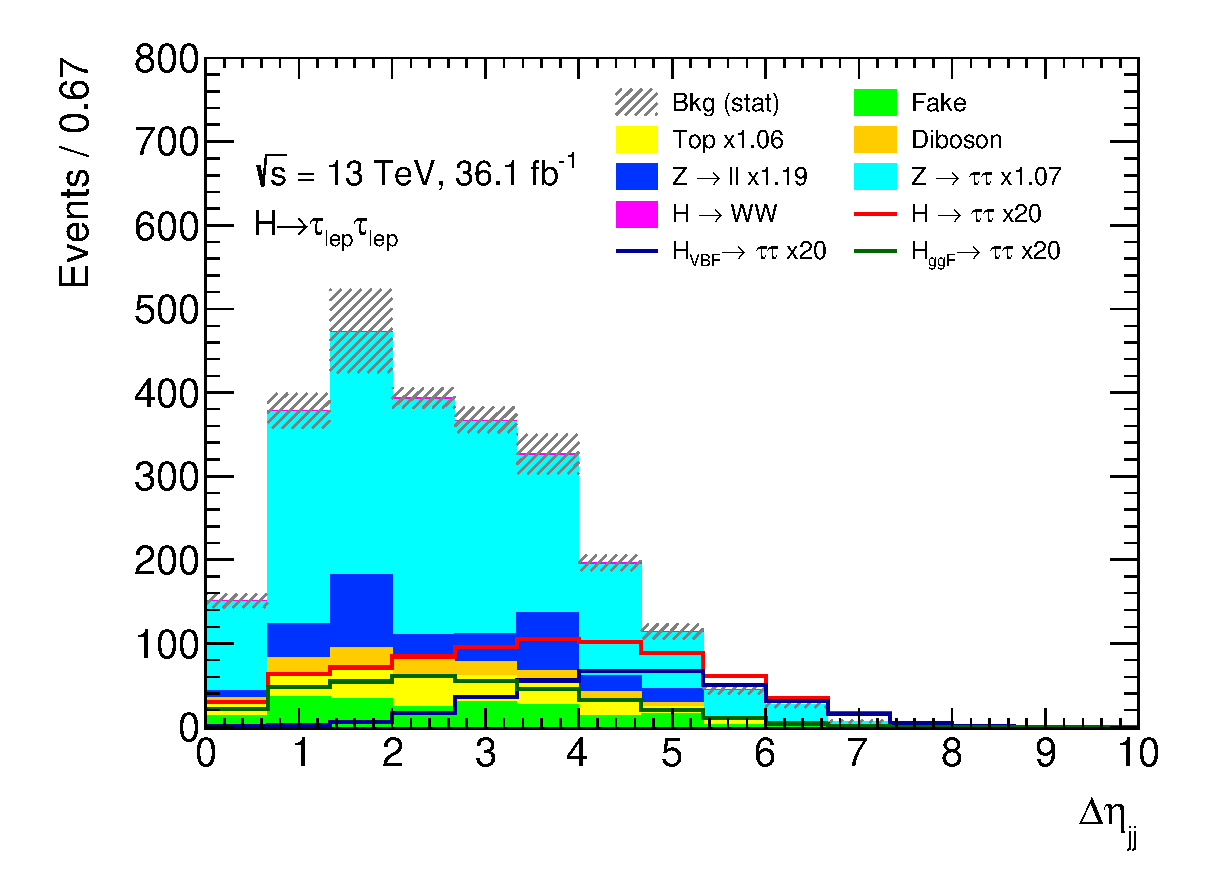
\includegraphics[width=\textwidth]{./plots/event_selection/categories/ll-CutVBFCatOppositeHemispheres-DJetEta-lin.eps}
        \caption{}\label{fig:event_selection:cutflow:vbf:detajj}
    \end{subfigure}
    \begin{subfigure}[t]{0.45\textwidth}
        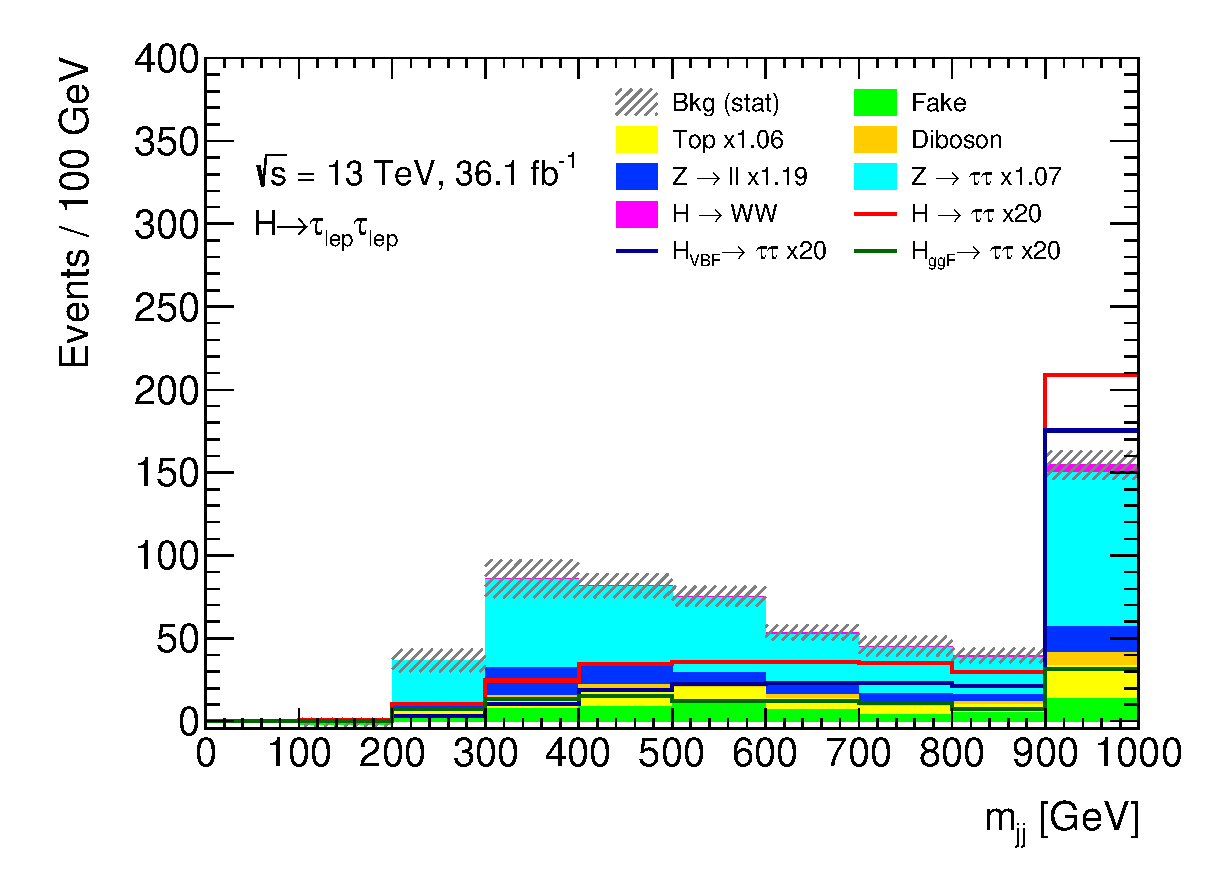
\includegraphics[width=\textwidth]{./plots/event_selection/categories/ll-CutVBFCatLCentrality-Mjj-lin.eps}
        \caption{}\label{fig:event_selection:cutflow:vbf:mjj}
    \end{subfigure}
    \begin{subfigure}[t]{0.45\textwidth}
        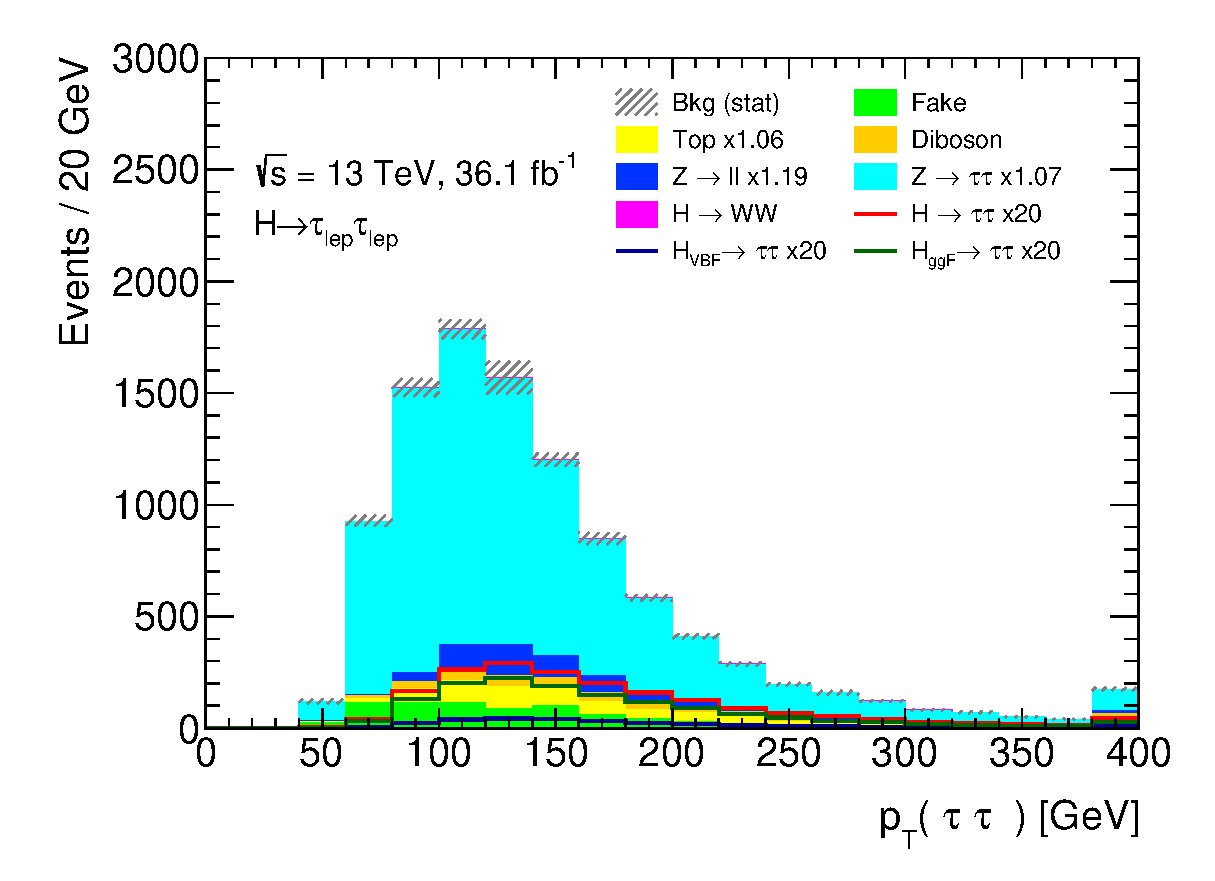
\includegraphics[width=\textwidth]{./plots/event_selection/categories/ll-CutBoostedCatNoVBF-PtTauTau-lin.eps}
        \caption{}\label{fig:event_selection:cutflow:boosted:pttautau}
    \end{subfigure}
    \caption{Distribution of several variables which are used in the categorization before the corresponding cut is applied.
             The following distributions are shown: $\pt^{\text{jet}_2}$ after Cut~16 (a, the first bin contains all events with no second jet),
             $\eta_{\text{jet}_1} \cdot \eta_{\text{jet}_2}$ after Cut~1V, $\detajj$ after Cut~2V, $m_{jj}$ after Cut~4V, and $\pt^{\tau\tau}$ after Cut~1B.
             The signal and background distributions are normalized to their theory cross-section and luminosity.
             Additional normalization factors are applied on the top-quark, $\Zll$, and $\Ztautau$ background.
             The signal is scaled by a factor of 20 for visibility.
             Underflow and overflow bins are included in the first and last bin, respectively.
             Only statistical uncertainties are included in the error band.}\label{fig:event_selection:categories}
\end{figure}


% \cref{fig:event_selection:boosted:mmc} shows the distributions of $\mmc$ in the inclusive boosted, low-boosted, and high-boosted regions.

% \begin{figure}[htb]
%     \centering
%     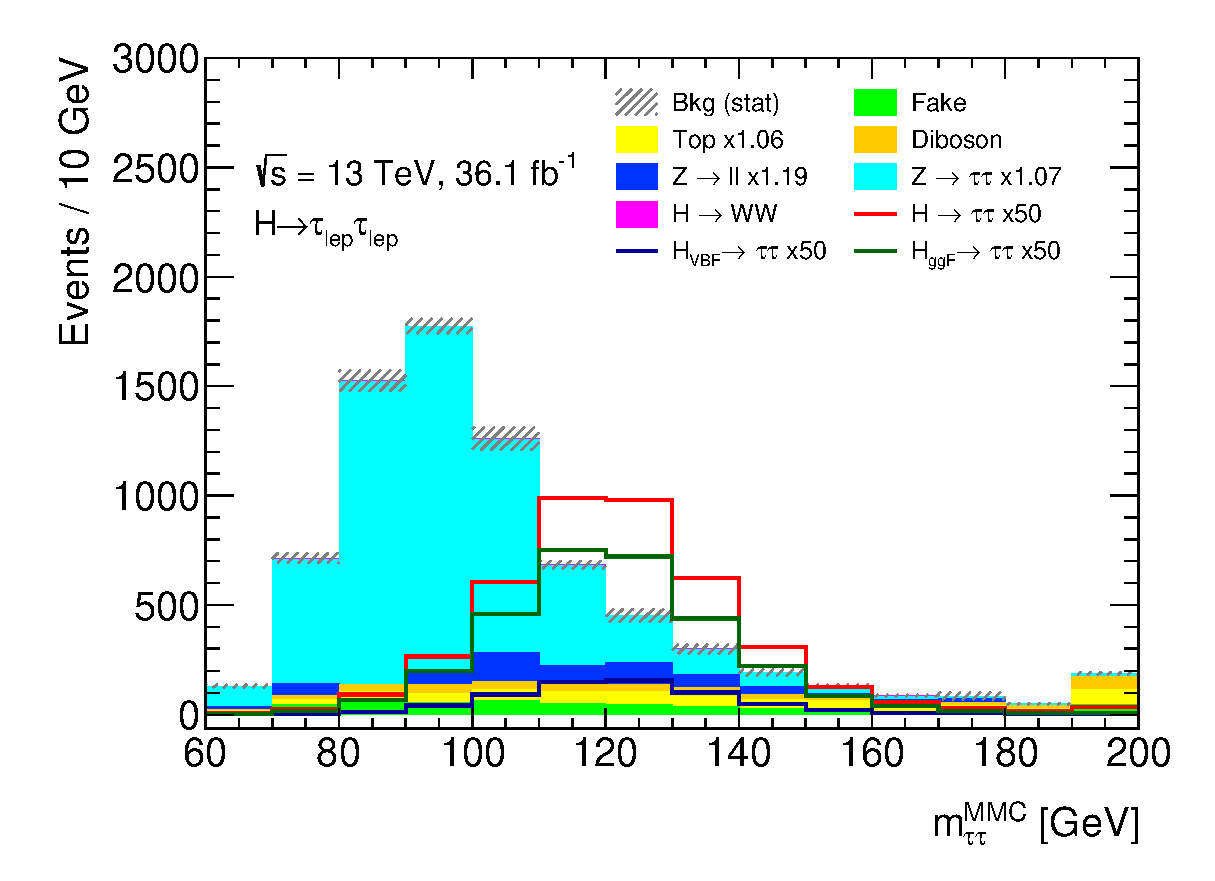
\includegraphics[width=0.3\textwidth]{./plots/event_selection/presel/ll-CutBoostedCatHiggsPt-dilep_mmc_mlm_m-lin.eps}
%     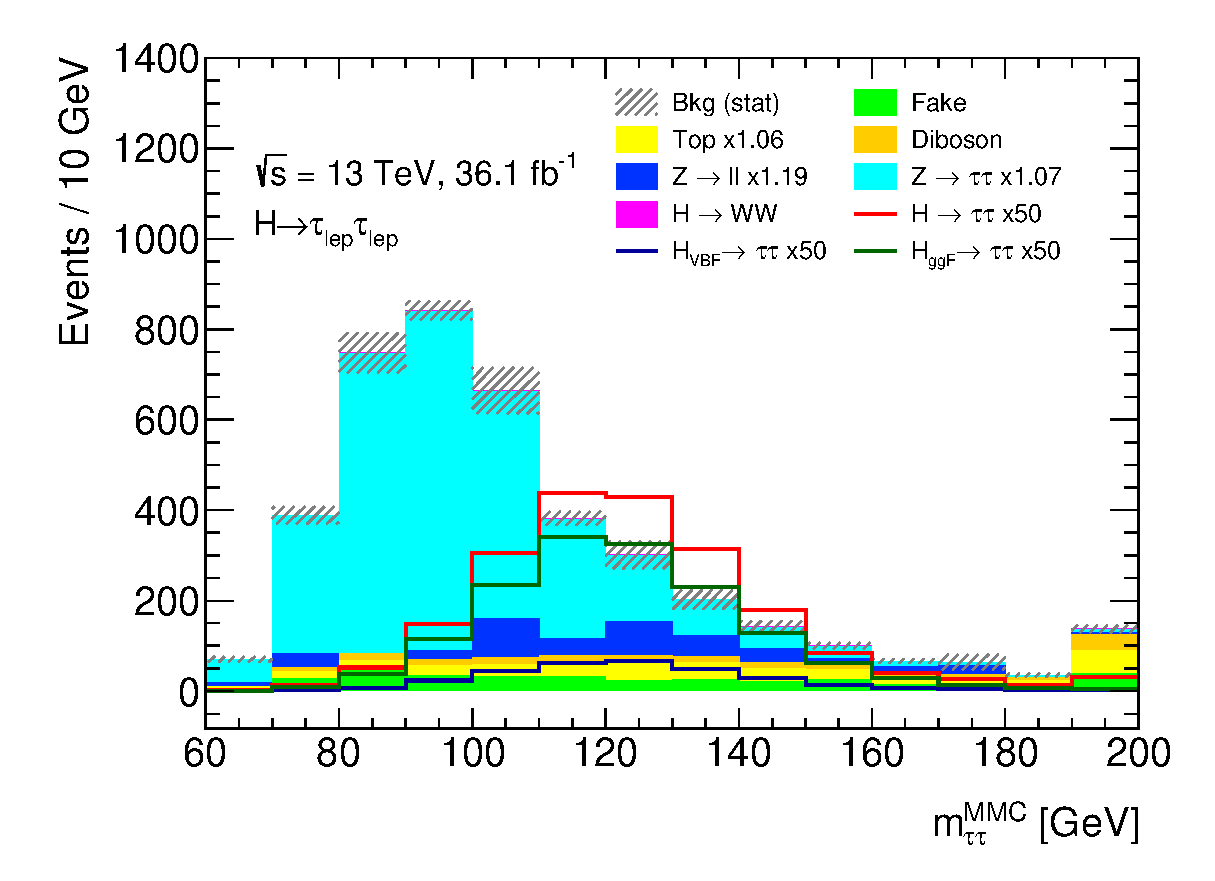
\includegraphics[width=0.3\textwidth]{./plots/event_selection/presel/ll-CutBoostedCatA-dilep_mmc_mlm_m-lin.eps}
%     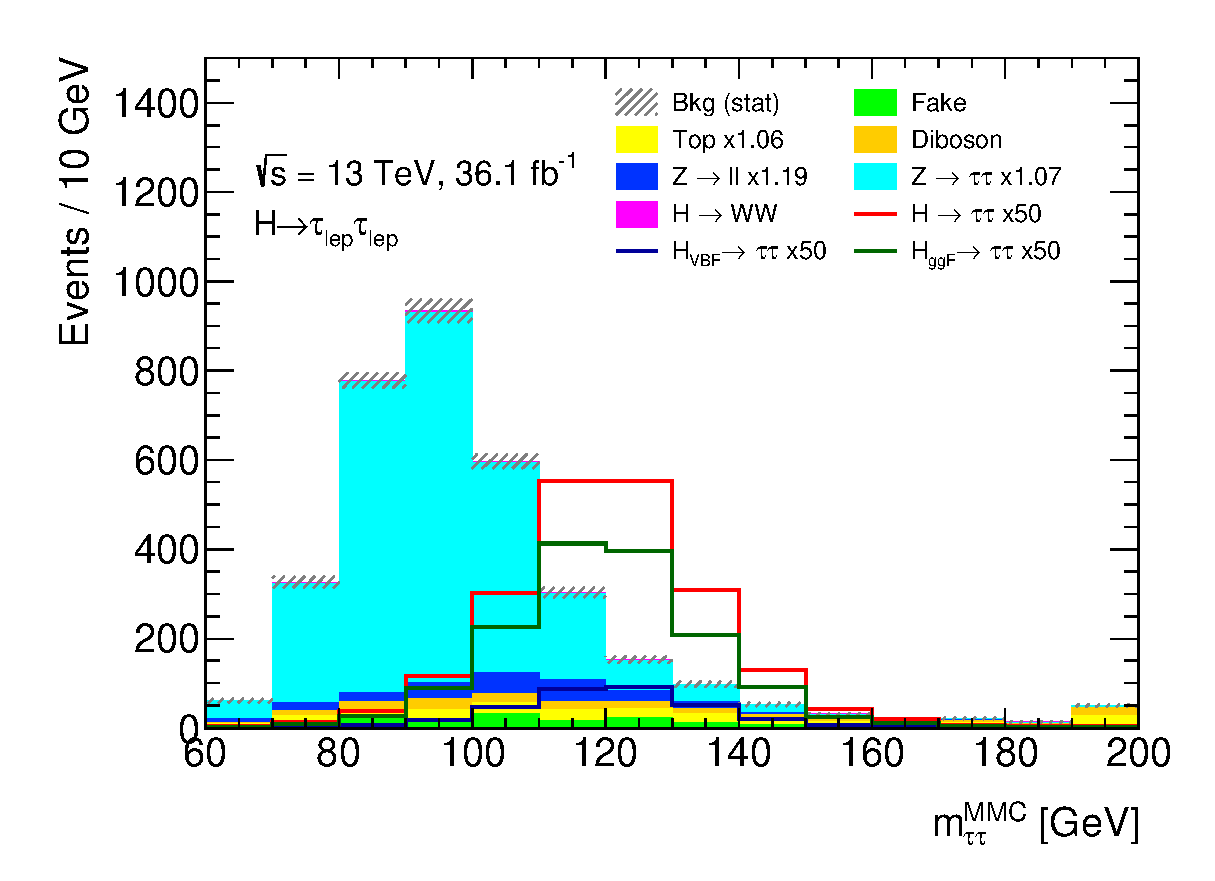
\includegraphics[width=0.3\textwidth]{./plots/event_selection/presel/ll-CutBoostedCatB-dilep_mmc_mlm_m-lin.eps}
%     \caption{Distributions of the output of the missing mass calculator algorithm, $\mmc$, in the inclusive boosted (left),
%              low-boosted (middle), and high-boosted (right) boosted category.
%              Normalization factors are applied on the top-quark, $\Zll$, and $\Ztautau$ background.
%              The signal is scaled by a factor of 20.
%              The error band includes statistic and systematic uncertainties.}\label{fig:event_selection:boosted:mmc}
% \end{figure}

\section{Event yields}\label{sec:event_selection:yields}

The event yields for the different signal and background processes after
the preselection and in the inclusive VBF and boosted categories are shown in \cref{tab:event_selection:yields}.
After the preselection the fraction of signal events is \SI{1.05}{\percent}.
For events from the ggF and VBF production mode the fractions are \SI{0.67}{\percent} and \SI{0.27}{\percent}, respectively.

In the VBF category the proportion of the VBF $\Htt$ process increases to \SI{2.65}{\percent}, but also the ggF production mode
contributes now \SI{0.93}{\percent}.
The overall contribution signal events to the total event count is \SI{3.63}{\percent}.

It was also possible to enhance the signal fraction in the boosted category.
The total signal contribution increases to \SI{1.09}{\percent}.
The proportions of the ggF and VBF production mode are \SI{0.79}{\percent} and \SI{0.12}{\percent}.
The fraction of VBF events is slightly worse than after the preselection, because most VBF events fell in the VBF category.

A large fraction of background events was rejected in the VBF category compared to the boosted category.
This can be explained by the distinct event topology of a VBF event, which makes it easier to separate signal and background events.

The most dominant background is the $\Zgammatt$ background with \SI{56}{\percent} (\SI{72}{\percent}) contribution for the
VBF (boosted) category, followed by the
$\Zgammall$ and top-quark background with a fraction of \SI{12}{\percent} (\SI{7}{\percent}) and \SI{11}{\percent} (\SI{7}{\percent}), respectively.
The QCD multijet (``fake'') background has a contribution of \SI{11}{\percent} in the VBF category and \SI{0.7}{\percent} in the boosted category.

\begin{table}[htpb]
    \centering
    \caption{Event yields for the different signal and background processes after the preselection
             and in the inclusive VBF and boosted categories with a combined 2016 and 2016 dataset of $\SI{36.1}{\invfb}$.
             Normalization factors are applied on the top-quark, $\Zll$, and $\Ztautau$ background.
             Only statistical uncertainties are shown.}\label{tab:event_selection:yields}
    \begin{tabular}{@{}l@{}
                    S[separate-uncertainty,table-figures-uncertainty=1]
                    S[separate-uncertainty,table-figures-uncertainty=1]
                    S[separate-uncertainty,table-figures-uncertainty=1]
                    @{}}
        \toprule
        Process             & {Preselection} & {VBF category} & {Boosted category} \\ \midrule
        ggF $\Htt$          & 74.17 \pm 0.55    &  5.18 \pm 0.15    & 60.71 \pm 0.49 \\
        VBF $\Htt$          & 28.97 \pm 0.15    & 14.77 \pm 0.10      & 12.88 \pm 0.10 \\
        WH  $\Htt$          &  5.48 \pm 0.20    &  0.10 \pm 0.02      & 4.94 \pm 0.19 \\
        ZH  $\Htt$          &  2.91 \pm 0.12    &  0.04 \pm 0.01      & 2.67 \pm 0.11 \\
        ttH $\Htt$          & 2.32 \pm 0.20     &  0.12 \pm 0.05      & 2.12 \pm 0.19 \\ \midrule
        Fakes               & 841.34\pm 31.75   & 59.06 \pm 8.83      & 529.25 \pm 26.28 \\
        Top                 & 684.23\pm 11.79   & 60.42 \pm 3.36      & 540.07 \pm 10.66 \\
        Diboson             & 438.00\pm 5.43    & 21.55 \pm 1.10      & 368.10 \pm 4.51 \\
        $\Zgammall$         & 684.86\pm 85.54   & 64.73 \pm 12.96     & 567.98 \pm 79.12 \\
        $\Zgammatt$         & 7992.32\pm 62.85  & 322.03 \pm 10.52    & 5541.34 \pm 50.81 \\
        $\HWW$              & 46.36\pm1.20      & 8.66 \pm 0.36       & 32.63 \pm 1.07 \\ \midrule
        Total signal        & 113.85\pm 0.65    & 20.21 \pm 0.19    & 83.33 \pm 0.58 \\
        Total background    & 10687.11\pm 111.56& 536.45 \pm 19.21    & 7579.37 \pm 98.33 \\ \bottomrule
        % Data                & 10630             & 489 & 7522 \\ \bottomrule
    \end{tabular}
\end{table}
